%%
%% Journal extension of the PIWM conference paper.
%% "Physically Interpretable World Models via Weakly Supervised
%%  Representation Learning" (conference) -> journal version.
%%
%% This journal version extends the conference paper along three axes:
%%   (1) two new partially observable driving case studies
%%       -- simulated CarRacing and a real physical DonkeyCar;
%%   (2) physically interpretable encoding of the external road environment;
%%   (3) physically interpretable prediction of the road environment.
%%
\documentclass[preprint,12pt]{elsarticle}

\usepackage{amsmath}
\usepackage{amssymb}
\usepackage{amsthm}
\usepackage{graphicx}
\usepackage{subcaption}
\captionsetup{font=small,labelfont=bf}
\usepackage[section]{placeins}
\usepackage{booktabs}
\usepackage{algorithm}
\usepackage{algpseudocode}
\usepackage{siunitx}
%% Without this, the .bbl falls back to \texttt for URLs, which cannot break
%% and pushes two ScienceDirect links ~75pt past the right margin.
\usepackage{url}
\usepackage{tikz}
\usetikzlibrary{arrows.meta,positioning,fit,calc,backgrounds}
%% Shared palette for the TikZ schematics; frenetink matches the "ours" curve
%% colour of the result figures (see src/paper_style.py, COL["Frenet"]).
\definecolor{frenetink}{HTML}{3B33A0}
\definecolor{previewor}{HTML}{E8820C}
%% Without these the document falls back to bitmap (Type 3) EC fonts, which look
%% ragged on screen, bloat the PDF, and are rejected by some production systems.
%% Latin Modern is metric-compatible with Computer Modern, so nothing reflows.
\usepackage[T1]{fontenc}
\usepackage{lmodern}
%% Character protrusion and font expansion: tightens justification, removes most
%% of the residual overfull boxes, and evens out the greyness of the text block.
%% Requires scalable fonts, hence lmodern above.
\usepackage{microtype}

%% Every figure asset lives in imgs/, so this directory is self-contained.
%% Elsevier's Editorial Manager flattens the uploaded file set, which breaks
%% any \includegraphics that reaches outside the manuscript directory.
\graphicspath{{imgs/}}

%% Long DOIs/URLs in the bibliography otherwise overflow the text block.
\emergencystretch=3em

%% Never strand a single line of a paragraph at the top or bottom of a page.
\widowpenalty=10000
\clubpenalty=10000

%% The results section is float-dense (3 figures + 3 tables in a few pages).
%% With LaTeX's defaults (max 2 top floats, max 3 floats/page, >=20% text per
%% page) the queue backs up and every figure is deferred past the bibliography.
\setcounter{topnumber}{3}
\setcounter{bottomnumber}{2}
\setcounter{totalnumber}{4}
\renewcommand{\topfraction}{0.9}
\renewcommand{\bottomfraction}{0.8}
\renewcommand{\textfraction}{0.07}
\renewcommand{\floatpagefraction}{0.7}

\newtheorem{definition}{Definition}
\newtheorem{problem}{Problem}
\renewcommand{\algorithmicrequire}{\textbf{Input:}}
\renewcommand{\algorithmicensure}{\textbf{Output:}}

% Convenience macros for the factorized interpretable state.
\newcommand{\zv}{z^{v}}      % vehicle-relative state
\newcommand{\zr}{z^{r}}      % road-context state
\newcommand{\zstar}{z^{*}}   % interpretable state

\journal{Robotics and Autonomous Systems}

\begin{document}

\begin{frontmatter}

\title{Physically Interpretable World Models for Partially Observable
       Driving: Encoding and Predicting the Road Environment under
       Weak Supervision}

%% ---------------------------------------------------------------
%% TODO(authors) --- FILL IN BEFORE SUBMISSION.
%% The placeholder \author below exists only so that the \affiliation
%% has something to attach to; without any \author, elsarticle typesets
%% the title followed by an orphan address block and no byline.
%% The conference version (arXiv:2412.12870) is authored by
%%   Zhenjiang Mao, Mrinall Eashaan Umasudhan, Ivan Ruchkin.
%% Confirm the journal author list, order, corresponding author and
%% e-mail, then replace the placeholder with the block below.
%%
%% \author[uf]{First Author}
%% \author[uf]{Second Author}
%% \author[uf]{Corresponding Author\corref{cor1}}
%% \ead{corresponding@ufl.edu}
%% \cortext[cor1]{Corresponding author.}
%% ---------------------------------------------------------------
\author[uf]{[AUTHOR LIST --- TO BE COMPLETED BEFORE SUBMISSION]}

\affiliation[uf]{organization={Trustworthy Engineered Autonomy (TEA) Lab,
                               University of Florida},
               city={Gainesville},
               state={Florida},
               country={USA}}

%% ---------------------------------------------------------------
\begin{abstract}
Learning predictive models from high-dimensional observations is fundamental for
safe autonomous cyber-physical systems, yet the latent states of standard world
models lack physical interpretability.
Our conference work introduced the Physically Interpretable World Model (PIWM),
which aligns latent representations with physical quantities and constrains
their evolution through partially known dynamics under distribution-based weak
supervision.
That formulation assumes the vehicle state is a complete Markov description of
the task, which holds for fully observable benchmarks such as CartPole and Lunar
Lander but fails for driving: two vehicles with identical position, heading and
speed follow divergent futures when the road ahead differs, and a forward-facing
camera reveals that road only partially.
This article extends PIWM to partially observable driving along three axes.
First, we move to two partially observable driving case studies: a simulated
top-down \emph{CarRacing} track and a \emph{real, physical DonkeyCar}.
Second, we introduce a physically interpretable \emph{encoding} of the road
environment, factorizing the interpretable latent into a vehicle-relative
component and a road-context component---lateral deviation, vehicle--road
heading error and curvature---inferred from onboard images.
Third, we introduce a physically interpretable \emph{prediction} of that
environment: a split-dynamics model that advances the vehicle through structured
kinematics while forecasting how the road context evolves.
On the physical DonkeyCar, where road context is supervised only during training
and must be recovered from the front camera at test time, PIWM attains
\SI{0.463}{m} position error over a 100-step rollout against \SI{0.703}{m} for
the strongest baseline under five-fold cross-validation, ahead in every fold, with
less than half the fold-to-fold variation of any baseline---and with every state
variable physically meaningful.
\end{abstract}

\begin{keyword}
physically interpretable world models \sep partial observability \sep
autonomous driving \sep road-context encoding \sep weak supervision \sep
trajectory prediction
\end{keyword}

\end{frontmatter}

%% ==============================================================
\section{Introduction}\label{sec:intro}
%% ==============================================================

Accurate and robust trajectory prediction from high-dimensional sensor data
is a foundational challenge for autonomous cyber-physical systems (CPS).
Modern \emph{world models}~\cite{ha2018world} address this challenge by
encoding observations into compact latent representations and predicting their
temporal evolution, a paradigm that has proven effective for long-horizon
prediction, planning, and control~\cite{micheli2022transformers,
hafner2023mastering, seo2023masked}.
Despite strong empirical performance, the latent states of these models
typically lack a clear connection to the underlying physical state of the
system.
In safety-critical settings such as autonomous driving and robotics, this
opacity limits trustworthiness: without interpretable states, it is difficult
to detect unsafe future configurations, diagnose prediction failures, or apply
formal safety-monitoring techniques~\cite{hasan2015formal, katz2022verification,
alshiekh2018safe}.

Our prior conference work introduced the Physically Interpretable World Model
(PIWM)~\cite{piwm_conf}, a framework that aligns latent representations with
physical quantities and constrains their temporal evolution through a partially
known dynamics model.
PIWM defines physical interpretability through two complementary properties:
the latent state must correspond to meaningful physical variables (state
semantics), and its temporal evolution must follow physically consistent
dynamics (temporal correctness).
A key feature of PIWM is \emph{distribution-based weak supervision}: rather than
requiring precise ground-truth state labels, the method accepts state estimates
in the form of sample distributions, as naturally produced by real-world sensing
pipelines such as GPS or radar.
Experiments on CartPole, Lunar Lander, and DonkeyCar demonstrated that
PIWM recovers accurate physical parameters and achieves long-horizon prediction
accuracy well beyond data-driven baselines.
A systematic comparison of intrinsic versus extrinsic architectures and
continuous versus discrete latent spaces showed that an extrinsic architecture
with a quantized (VQ-based) latent yields the most robust and physically grounded
representations.

\subsection*{The challenge: driving is partially observable}

Applying PIWM to realistic driving exposes a fundamental limitation of the
original formulation, and motivates the extensions in this article.
On CartPole and Lunar Lander, the system state completely specifies what will
happen next: the dynamics are fully observable and Markov, so a world model that
tracks the vehicle (or pole, or lander) state captures everything relevant to the
future.
Driving is different.
Consider two vehicles with identical position, heading, and speed.
If one is approaching a tight curve while the other is on a straight segment,
their future trajectories diverge even under the same control inputs.
The vehicle's physical state $x_t = (x, y, \psi, v)$ does not capture this
difference.
The missing information is the \emph{road context}: the shape of the lane ahead
(its curvature) and the vehicle's lateral and angular relationship to it, none of
which is part of any standard vehicle-state representation.
As a result, the vehicle state alone is \emph{non-Markov} with respect to future
motion: two identical states lead to different futures depending on the
unobserved road geometry.
Applying the original PIWM formulation to such tasks implicitly treats the
system as fully observable when it is not, causing the dynamics model to learn an
underdetermined, ill-posed mapping.

This challenge has two distinct facets, and overcoming each requires a separate
mechanism.
\emph{(i) The road environment must be encoded.}
The relevant road context is not given as a clean state vector; it is latent in
the pixels and, for a forward-facing camera, only partially visible at any
instant.
A physically interpretable driving world model must therefore \emph{infer} the
geometry of the surrounding road from raw images, and represent it in physically
meaningful terms rather than as opaque features.
\emph{(ii) The road environment must be predicted.}
Long-horizon rollout requires anticipating how the road context itself evolves as
the vehicle advances: the lane that is far ahead now becomes the lane the vehicle
is on a few steps later.
A world model that predicts only the vehicle state, treating the road as static
or as noise, accumulates error rapidly because it cannot anticipate the geometry
it is about to enter.
Predicting the road, like encoding it, should be physically interpretable so that
the forecasted environment can be inspected, trusted, and monitored.

These two facets, encoding and predicting the external environment, are
what distinguishes a driving world model from the vehicle-centric formulation of
the conference paper, which modeled only the state of the controlled body.
They are also why partial observability cannot be papered over by simply adding
capacity to a black-box predictor: the missing variable is structured, physical,
and causally upstream of the vehicle's future, so it deserves an explicit,
physically grounded treatment.

\subsection*{Our approach}

We resolve partial observability by reformulating the interpretable state as a
structured composition of two complementary components.
The \emph{vehicle-relative state} $\zv$ captures the ego vehicle's displacement
and heading change expressed in a local reference frame anchored at the beginning
of each prediction window; this representation removes dependence on global
coordinates and improves transferability across trajectories.
The \emph{road-context state} $\zr$ captures task-relevant environmental
structure: the cross-track error (lateral deviation from the lane center), the
vehicle--road heading error, and the local road curvature.
Together, $(\zv, \zr)$ form a Markov description of the driving task, restoring
the validity of the predictive world-model framework.
The vehicle-relative component is governed by a structured kinematic model whose
unknown actuation parameters are recovered during training; the road-context
component is governed by a geometry-driven transition that advects the road past
the vehicle as it advances, rather than treating the road as a free latent that
can drift.
This split-dynamics formulation provides appropriate inductive biases for each
component and decouples the faster-varying vehicle motion from the
slower-varying road context.

We validate the extended formulation in two new partially observable driving
environments.
In \textbf{CarRacing}, a top-down simulated racing environment, the road geometry
is present in the image but absent from the vehicle state; the model must learn to
infer and exploit road-context information from raw pixels.
On the physical \textbf{DonkeyCar} platform, a real RC-scale car observes its
environment through a front-facing camera and drives on a laboratory track.
During training, an external localization system provides ground-truth road
context as a privileged signal; at test time this signal is withheld, and the
model must infer and roll out road context solely from the onboard front-facing
image stream.
This setup tests whether the factorized representation learned under privileged
supervision transfers to the more challenging unaided real-world deployment
setting.
On the physical platform, over a 100-step ($\approx$\SI{4.5}{s}) rollout and under
five-fold cross-validation, PIWM with factorized state and split dynamics reaches
\SI{0.463}{m} position error against \SI{0.703}{m} for the strongest data-driven
or physics-informed baseline, ahead in every fold, and the gap widens with the
horizon: the baselines diverge while PIWM stays bounded.

\subsection*{Contributions}

This journal article extends the conference version~\cite{piwm_conf}
along three axes, which constitute its three contributions.

\begin{enumerate}
    \item \textbf{Two partially observable driving case studies.}
    We move PIWM beyond the fully observable benchmarks of the conference paper
    to two new driving environments that are genuinely partially observable:
    a simulated top-down \emph{CarRacing} track and a \emph{real, physical
    DonkeyCar} platform driven on a laboratory track under onboard-camera
    observation.
    We formally characterize partial observability in driving, showing that the
    vehicle state is non-Markov with respect to future trajectory, and use these
    two case studies to demonstrate the practical consequences and the benefit of
    the proposed treatment.

    \item \textbf{Physically interpretable encoding of the road environment.}
    Unlike the conference formulation, which modeled only the controlled body's
    state, we model the \emph{external environment}.
    We introduce a factorization of the interpretable latent into a
    vehicle-relative component $\zv$ and a road-context component $\zr$, where
    $\zr$ comprises physically meaningful descriptors of the road (cross-track
    error, vehicle--road heading error, and curvature).
    We show how to infer $\zr$ from images using temporal context, including the
    forward-camera case where the road ahead is only partially visible, and how
    privileged supervision available only at training time can be used to learn
    this encoding.

    \item \textbf{Physically interpretable prediction of the road environment.}
    We introduce a split-dynamics model that not only rolls out the vehicle with
    a structured kinematic model, but also \emph{forecasts the road context} with
    a geometry-driven transition in which the road is advected past the vehicle
    by its own predicted motion.
    The predicted road context is itself physically interpretable, so the
    forecasted environment, not just the forecasted vehicle, can be inspected and
    monitored.
    We show that this geometric treatment, rather than propagating the road as a
    free latent, is what keeps long-horizon rollout bounded, and that the road
    context can be perceived from the onboard camera at a cost of roughly
    \SI{2}{cm} in \num{100}-step position error relative to a privileged map
    lookup.
\end{enumerate}

\noindent
The remainder of this article is organized as follows.
Section~\ref{sec:related} surveys related work.
Section~\ref{sec:preliminaries} reviews background on autonomous CPS, world
models, and physical interpretability.
Section~\ref{sec:problem} formalizes the partial observability problem in driving
and introduces the factorized state.
Section~\ref{sec:architecture} presents the PIWM architecture, the road-context
encoder (Section~\ref{sec:encoding}), and the road-context predictor
(Section~\ref{sec:prediction}).
Section~\ref{sec:experiments} describes the experimental setup, and
Section~\ref{sec:results} reports results on the benchmarks and on the real
DonkeyCar.
Section~\ref{sec:discussion} discusses implications and limitations, and
Section~\ref{sec:conclusion} concludes.


%% ==============================================================
\section{Related Work}\label{sec:related}
%% ==============================================================

We organize the discussion into five threads relevant to physically interpretable
world modeling under partial observability: trajectory prediction and safe forecasting
(Section~\ref{sec:rw_traj}), representation learning for dynamical systems
(Section~\ref{sec:rw_repr}), world models (Section~\ref{sec:rw_wm}),
physics-informed and interpretable learning (Section~\ref{sec:rw_phys}), and
partial observability, privileged learning, and road structure
(Section~\ref{sec:rw_po}).
We close each thread by positioning PIWM against it.

\subsection{Trajectory Prediction and Safe Forecasting}\label{sec:rw_traj}

Predicting future motion is central to safe planning and
control~\cite{fridovich2020confidence}.
Classical predictors propagate a low-dimensional state with hand-specified
models: Kalman-filter formulations over a bicycle model of vehicle
motion~\cite{ammoun2009real}, and Hamilton--Jacobi reachability for sets of
reachable states with formal guarantees~\cite{li2021prediction,
nakamura2023online, muthali2023multi}.
These methods are transparent and certifiable, but they require an explicit
dynamical model and a low-dimensional state, and they scale poorly to
high-dimensional camera observations.

Learning-based predictors instead forecast directly from data.
Social-pooling and generative sequence models capture multi-agent
interaction~\cite{alahi2016social, gupta2018social, wen2022social}, while graph-
and attention-based models such as Trajectron++ achieve strong forecasting by
conditioning on scene graphs and high-definition maps~\cite{salzmann2020trajectron++}.
Hybrid schemes embed classical filters inside learned models, as in learned
Kalman filtering~\cite{revach2022kalmannet}.
These models, however, depend on handcrafted scene representations or HD-map
annotations that are unavailable in many settings~\cite{itkina2023interpretable,
hsu2023interpretable}, and their internal states carry no physical meaning.

A parallel line equips predictors with reliability guarantees without altering
the predictor itself: conformal prediction and calibrated forecasting bound error
or coverage~\cite{lindemann2023conformal, lu2024towards, ruchkin2022confidence,
cleaveland2022risk}; statistical model checking and predictive monitoring estimate
the probability of property violations~\cite{qin2022statistical, zarei2020statistical,
cairoli2021neural, waga2022dynamic}; and runtime and misbehavior monitors flag
unsafe behavior online~\cite{stocco2020misbehaviour, ma2020stlnet, mao2024safe,
mao2025safe}.
These techniques are complementary to ours: they wrap a predictor with guarantees
but do not make its latent state physically meaningful.
Compared with this body of work, PIWM learns interpretable representations
directly from raw images under weak supervision, without handcrafted scene
representations or test-time state labels, so that the forecast itself, both the
vehicle and the road around it, can be inspected.

\subsection{Representation Learning for Dynamical Systems}\label{sec:rw_repr}

Compact latent representations underpin learning from high-dimensional
observations, from classical autoencoders~\cite{Hinton06} to variational
autoencoders (VAEs)~\cite{kingma2013auto}, but standard objectives impose no
physically meaningful structure.
A large literature seeks more structured latents by encouraging
disentanglement~\cite{higgins2017beta, kim2018disentangling, chen2018isolating},
causal structure~\cite{yang2021causalvae, scholkopf2021toward}, or object-centric
and slot decompositions~\cite{mosbach2025soldslotobjectcentriclatent}.
Discrete VQ-VAEs regularize the latent through a learned
codebook~\cite{van2017neural, razavi2019generating}; PIWM builds on this
quantization but, unlike it, ties codebook components to physical values.
These methods improve organization or modularity, yet none guarantees
correspondence to measurable physical quantities.

Closer to physical grounding, several models steer latents toward physics.
GOKU-net constrains the latent dynamics to a known ODE and infers that ODE's
parameters~\cite{linial_generative_2021}, but the functional form must be fixed a
priori and the latents are tied to it rather than to quantities that can be
measured from the observation; SPARTAN produces
semantically structured outputs but incorporates neither known dynamics nor
action-conditioned prediction~\cite{lei2024spartan}; Deep Variational Bayes
Filters add latent state-space dynamics to VAEs and report latents that correlate
with physical quantities~\cite{karl2016deep}, but the correspondence emerges from
the transition structure rather than being enforced, so which dimension carries
which quantity is not fixed in advance; and continuous-time models such as Neural
ODEs learn smooth but uninterpretable latent dynamics~\cite{chen2018neural}.
Representation learning specialized for pixel-based control has been studied
extensively for its effect on downstream
performance~\cite{tomar2021learningrepresentationspixelbasedcontrol}, while again
leaving the latent opaque.
Compared with these approaches, PIWM explicitly aligns latent dimensions with
named physical quantities of both the vehicle and the surrounding road, and
constrains their evolution with known physics under only weak, distribution-based
supervision.

\subsection{World Models}\label{sec:rw_wm}

World models learn latent dynamics for imagination-based planning and control.
The Dreamer and PlaNet line learns recurrent latent state-space models from
pixels~\cite{hafner2019learning, hafner2020mastering, hafner2023mastering};
transformer- and masked-prediction world models improve sample
efficiency~\cite{micheli2022transformers, seo2023masked}, and the same family has
been trained directly on physical robots~\cite{wu2023daydreamer}; and a range of
variants explore alternative latent
factorizations~\cite{ha2018world, zhang2021world, zhao2024decomposed}.
These models excel empirically but learn latent spaces with no clear physical
meaning, which limits inspection and safety monitoring.

For driving, recent world models predict rich structured futures such as 3D
occupancy grids or rendered scenes~\cite{zheng2024occworld, min2023uniworld,
yan2024renderworld, zuo2024gaussianworld}, improving forecasting realism but still
without aligning the internal state to physical variables.
Neuro-symbolic world models improve generalization, but their symbolic vocabulary
is either supplied in advance or induced separately from the physical
quantities a controller acts on~\cite{balloch2023neuro, liang2024visualpredicator}.
The closest prior work, Vid2Param, recovers physical parameters from
video~\cite{asenov2019vid2param} but requires full supervision and provides no
explicit world model for long-horizon rollout.
Compared with these approaches, PIWM recovers physical state under weak
supervision and rolls it forward through interpretable dynamics, and, new in this
article, it does so for the external road environment, not only the controlled
body.

\subsection{Physics-Informed and Interpretable Learning}\label{sec:rw_phys}

A complementary thread injects physics directly into learning.
Sparse identification of nonlinear dynamics and differentiable-physics or
end-to-end system identification recover governing equations or
parameters~\cite{BRUNTON2016710, de2018end, yao2024marrying}, while
physics-informed neural networks embed differential constraints in the
loss~\cite{cai2021physics, ZHONG2023115664}.
Within world modeling, physical priors have been added as bounds on states and
actions~\cite{tumu2023physics, sridhar2023guaranteed}, as known physics entering
the model's drift term as an inductive bias~\cite{djeumou2023learn},
kinematics-inspired layers~\cite{cui2020deep}, and
Taylor-monomial-structured latent dynamics (Phy-Taylor)~\cite{mao_phy-taylor_2025}.

Most of these methods assume access to the underlying low-dimensional state and
are not designed for raw visual inputs, or they enforce physical plausibility
without yielding a state that names specific quantities.
PIWM differs in two ways aligned with this article's contributions: it extracts
the physical state from images under weak supervision, so that physics can be
applied without ground-truth labels, and it applies a structured, learnable
physical model, a bicycle model for the vehicle and a geometry-driven transition
for the road, to roll the interpretable state forward.
Compared with physics-informed predictors that model only the controlled body,
PIWM applies interpretable physical structure to the external environment as well.

\subsection{Partial Observability, Privileged Learning, and Road Structure}\label{sec:rw_po}

Partial observability is a long-standing challenge in robotics and reinforcement
learning, classically formalized through partially observable Markov decision
processes and belief-state planning~\cite{kaelbling1998planning,
kaelbling1996reinforcement}.
Model-free agents commonly cope with it by adding memory through recurrent or
temporal architectures: recurrent policy gradients~\cite{wierstra2007solving},
gated recurrent networks~\cite{chung2014empirical}, convolutional LSTMs for
spatiotemporal inputs~\cite{shi2015convolutional}, and temporal convolutional
networks~\cite{bai2018empirical}.
These approaches recover an opaque belief or memory state; they do not produce a
physically interpretable estimate of the missing environmental variables, which is
exactly what our road-context state provides.

When information needed for learning is available only at training time,
privileged-information and teacher--student learning supervise a model that must
operate without it at deployment~\cite{chen2020learning, gou2021knowledge}.
This is the mechanism we use on the real DonkeyCar: ground-truth road context from
training-time track localization teaches the encoder what to extract, while the
deployed car observes only its front camera and must reconstruct that context from
images.

In driving specifically, a substantial literature encodes lane and road structure
in learned representations~\cite{salzmann2020trajectron++, itkina2023interpretable},
but typically requires explicit maps or HD annotations; and physics-based
predictors apply kinematic or dynamic bicycle models to low-dimensional state
vectors~\cite{kong2015kinematic} rather than to learned image representations.
Learning-based control has also been demonstrated on RC-scale physical cars,
including reinforcement learning on the DonkeyCar
platform~\cite{viitala2021learning}, but without an
interpretable predictive world model.
Compared with all of the above, our work is, to our knowledge, the first to
integrate a factorized vehicle--road representation with a physics-informed world
model trained from images under weak supervision, and to both \emph{encode} and
\emph{predict} the road environment in physically interpretable terms.


%% ==============================================================
\section{Preliminaries}\label{sec:preliminaries}
%% ==============================================================

\subsection{Autonomous CPS and World Models}

\begin{definition}[Autonomous CPS]
An \emph{autonomous CPS}, represented by the tuple $s = (X, I, Y, A, \phi_{\theta}, g, h)$, models the
evolution of an observation-based control system, where $X$ is the physical
state space, $I \subset X$ the set of initial states, $Y$ the observation space,
$A$ the action space, $\phi_{\theta}: X \times A \times \Theta \rightarrow X$ the
dynamics with unknown parameters $\theta \in \Theta$, $g: X \rightarrow Y$ the
observation function, and $h: Y \rightarrow A$ the controller.
\end{definition}

The true state evolves as $x_{t+1} = \phi(x_t, a_t, \theta^*)$, where $\theta^*$
are the unknown true parameters.
The controller selects actions from observations: $a_t = h(y_t) = h(g(x_t))$.
A world model serves as a learned surrogate for forecasting future observations.

\begin{definition}[World Model]
A \emph{world model} $\mathcal{W} = (\mathcal{E}, f, \mathcal{D})$ predicts the
future evolution of observations in an autonomous CPS $s$, where
$\mathcal{E}: Y \rightarrow Z$ encodes observations into latent representations,
$f: Z \times A \rightarrow Z$ predicts future latents, and
$\mathcal{D}: Z \rightarrow Y$ reconstructs predicted observations.
\end{definition}

Conventional world models are evaluated by predictive accuracy in image space
(e.g., MSE or SSIM).
However, low image error does not imply that the underlying predicted state is
physically meaningful: similar-looking frames can correspond to very different
physical configurations.
For safety monitoring and planning, what matters is not only visual fidelity but
whether the latent state can be interpreted as a physical quantity and evolved
according to physically plausible dynamics.

\subsection{Physical Interpretability}

Following the conference paper~\cite{piwm_conf}, we define \emph{physical
interpretability} via two complementary properties:
\begin{enumerate}
    \item the latent representation $\zstar$ corresponds to meaningful physical
    variables (state semantics), and
    \item its temporal evolution follows physically consistent dynamics
    (temporal correctness).
\end{enumerate}
Property~1 requires alignment between the latent and the physical state, which
PIWM enforces through weak supervision.
Property~2 requires that multi-step rollouts of the latent state obey the known
equations of motion, which PIWM enforces through the structured dynamics model.

\begin{definition}[Interpretable Representation Learning Problem]
Given a dataset $\mathcal{S} = \{(y_{1:M}, a_{1:M}, \Xi_{1:M})\}_{1:N}$,
where $\Xi_t = \{\xi^{(l)}_t\}_{l=1}^L$ are samples drawn from an unknown
supervisory distribution $p(x_t)$, and a controller $h$, learn a latent encoder
$\mathcal{E}$ such that the mean squared error between the physical state $x_t$
and the encoded latent $\zstar_t = \mathcal{E}(y_t)$ is minimized:
\begin{equation}
    \min_{\mathcal{E}} \ \mathbb{E} \big[ \| x_t - \mathcal{E}(y_t) \|_2^2 \big].
\end{equation}
\end{definition}

The supervisory samples $\Xi_t$ are drawn from an unknown distribution $p(x_t)$
with no assumed parametric form; we only require that the distribution is
\emph{mean-proximal}, meaning its mean lies within a relative interval of width
$\delta$ around the true value (see Section~\ref{sec:setup} for the precise noise
model).
This is a strictly weaker assumption than standard supervised learning with
precise labels, and represents the uncertainty naturally arising from real-world
sensing.


%% ==============================================================
\section{Partial Observability in Driving}\label{sec:problem}  %% [NEW]
%% ==============================================================

This section formalizes the challenge introduced in Section~\ref{sec:intro}:
in driving, the vehicle state is not a sufficient statistic for the future.
The formalization motivates the factorized state that the rest of the article
encodes (Section~\ref{sec:encoding}) and predicts (Section~\ref{sec:prediction}).

\subsection{Why Vehicle State Is Insufficient for Driving}

The PIWM conference paper formulated physical interpretability under the implicit
assumption that the vehicle's physical state $x_t$ provides a complete, Markov
description of the system: knowing $x_t$ and action $a_t$ determines $x_{t+1}$.
This assumption holds for CartPole, Lunar Lander, and other low-dimensional
benchmark tasks, where the system state encodes all task-relevant information.
It fails for driving tasks.

In a driving task, the vehicle state $x_t = (x, y, \psi, v)$ (position, heading,
speed) does not encode the geometry of the road ahead.
The actual lane-following dynamics of the vehicle depend on this geometry:
\begin{equation}
    x_{t+1} = \phi(x_t,\; r_t,\; a_t,\; \theta^*),
    \label{eq:augmented_dyn}
\end{equation}
where $r_t$ denotes the \emph{road-context state}, which includes quantities such
as the lateral deviation from the lane center, the vehicle's heading relative to
the road tangent, and the local curvature.
The road-context component $r_t$ is not directly observed by the onboard camera
and is not part of any standard vehicle-state representation.

\begin{definition}[Partial Observability in Driving]
\label{def:partial_obs}
A driving task is \emph{partially observable} with respect to world modeling if
the vehicle state $x_t$ alone is not sufficient to determine future motion;
equivalently, if there exist two system configurations $(x_t, r_t^{(1)})$ and
$(x_t, r_t^{(2)})$ with $r_t^{(1)} \neq r_t^{(2)}$ such that, under the same
controller $h$, the resulting trajectories satisfy
$x_{t+1:T}^{(1)} \neq x_{t+1:T}^{(2)}$.
\end{definition}

The road-relative geometry is illustrated in Figure~\ref{fig:encoding}.
Two vehicles at identical positions on the track, with the same speed and
heading, enter different road segments (one straight, one curved).
Despite identical vehicle states and identical control actions, the predicted
future trajectories diverge, because the curvature of the upcoming road
introduces a lateral displacement that the vehicle-state-only dynamics cannot
anticipate.
Standard PIWM, which learns a single interpretable state aligned with $x_t$,
cannot represent this difference.
Two consequences follow, corresponding to the two facets of the challenge from
Section~\ref{sec:intro}: the model must \emph{encode} $r_t$ from observations
(Section~\ref{sec:encoding}), and it must \emph{predict} how $r_t$ evolves over
the horizon (Section~\ref{sec:prediction}).



\subsection{Factorized Interpretable State}\label{sec:factorized_state}

To resolve the partial observability problem, we augment the interpretable state
with road-context information and express the vehicle component in a translation-
and rotation-invariant reference frame.

\paragraph{Vehicle state}
Global coordinates $(x, y)$ introduce unnecessary dependence on the starting
position of each trajectory, complicating generalization across scenes.
In the road-aligned frame the vehicle's own motion is described by
\begin{equation}
    \zv_t =
    \begin{bmatrix}
        v_t \\ \omega_t
    \end{bmatrix},
    \label{eq:vehicle_rel}
\end{equation}
its longitudinal speed and yaw rate, both independent of where the trajectory
started.

\paragraph{Road-context state}
The road-context component $\zr_t$ captures the vehicle's configuration relative to
the road geometry:
\begin{equation}
    \zr_t =
    \begin{bmatrix}
        s_t \\ e_{\mathrm{CTE}} \\ e_{\psi}
    \end{bmatrix},
    \label{eq:road_ctx}
\end{equation}
where $s_t$ is the arc length travelled along the reference centerline,
$e_{\mathrm{CTE}}$ is the cross-track error (signed lateral distance from the lane
center) and $e_{\psi}$ is the heading error (difference between the vehicle's
heading and the road tangent at its current position).
Locating the vehicle by $s_t$ along the road rather than in the world is what
allows the road description below to be indexed by it.

\paragraph{Factorized state}
The complete \emph{factorized interpretable state} is
\begin{equation}
    \zstar_t = \left[ \zv_t,\; \zr_t \right]
             = \left( v_t,\, \omega_t,\, s_t,\, e_{\mathrm{CTE},t},\, e_{\psi,t} \right)
             \in \mathbb{R}^5 .
    \label{eq:factorized_state}
\end{equation}

The local curvature $\kappa$ is deliberately \emph{absent} from
\eqref{eq:factorized_state}: it is not propagated. The model instead carries a
curvature profile $\hat\kappa(\cdot)$ over arc length, perceived once from the
image window at the start of the rollout, and reads the curvature at the vehicle
from it,
\begin{equation}
    \kappa_t = \hat\kappa\!\left(s_t - s_{t_0}\right).
    \label{eq:kappa_readout}
\end{equation}
This distinction is what the rest of the article rests on. A model carrying
curvature as a state variable must predict how it evolves, and that prediction
compounds over a long rollout; re-indexing a profile observed once cannot compound,
because only the vehicle's position along the road advances.

The Markov property therefore holds for the pair
$\left(\zstar_t,\, \hat\kappa(\cdot)\right)$ with $\hat\kappa$ fixed across the
rollout: given the current factorized state, the perceived profile and the action,
the next factorized state is determined up to the unknown parameters $\theta^*$.
It does not hold for $\zstar_t$ alone, since~\eqref{eq:kappa_readout} requires the
profile.

\subsection{Extended Learning Problem}

The learning problem for partially observable driving extends the original PIWM
formulation as follows.

\begin{problem}[Interpretable State Learning under Partial Observability]
\label{def:po_problem}
Given a dataset
$\mathcal{S} = \{(y_{1:M},\, a_{1:M},\, \Xi^{v}_{1:M},\, \Xi^{r}_{1:M})\}_{1:N}$
where $\Xi^{v}_t$ and $\Xi^{r}_t$ are supervisory samples for the vehicle and
road-context components respectively, and a controller $h$, learn a factorized
physical encoder $\mathcal{E}_p$ whose two outputs
$(\zv_t, \zr_t) = \mathcal{E}_p(y_{1:t})$ approximate the vehicle state and the
road-context state, and which supports accurate future prediction under the task
dynamics.
\end{problem}

Two aspects distinguish this from the conference formulation, and they map
directly onto the two extensions developed next.
First, the encoder is conditioned on a \emph{history} $y_{1:t}$ rather than a
single frame: road context cannot be inferred from a single image (particularly
in the front-camera setting) and requires temporal context
(Section~\ref{sec:encoding}).
Second, the supervision is split: $\Xi^v_t$ can often be computed directly from
the vehicle state (available in simulation or via external localization), while
$\Xi^r_t$ requires knowledge of the road geometry.
In the real DonkeyCar experiments, road-context supervision is available only at
training time and withheld at test time, so the encoder must learn to recover
road context from images alone (Section~\ref{sec:encoding}), and the predictor
must roll it forward (Section~\ref{sec:prediction}).


%% ==============================================================
\section{PIWM Architecture}\label{sec:architecture}
%% ==============================================================

The PIWM architecture retains the core structure from the conference
version~\cite{piwm_conf}, comprising a physically interpretable autoencoder and a
learnable dynamics model, and extends it with the factorized state along two
axes: a road-context \emph{encoder} (Section~\ref{sec:encoding}) and a
road-context \emph{predictor} (Section~\ref{sec:prediction}).
A high-level overview is shown in Figure~\ref{fig:arch}.

\begin{figure}[t]
\centering
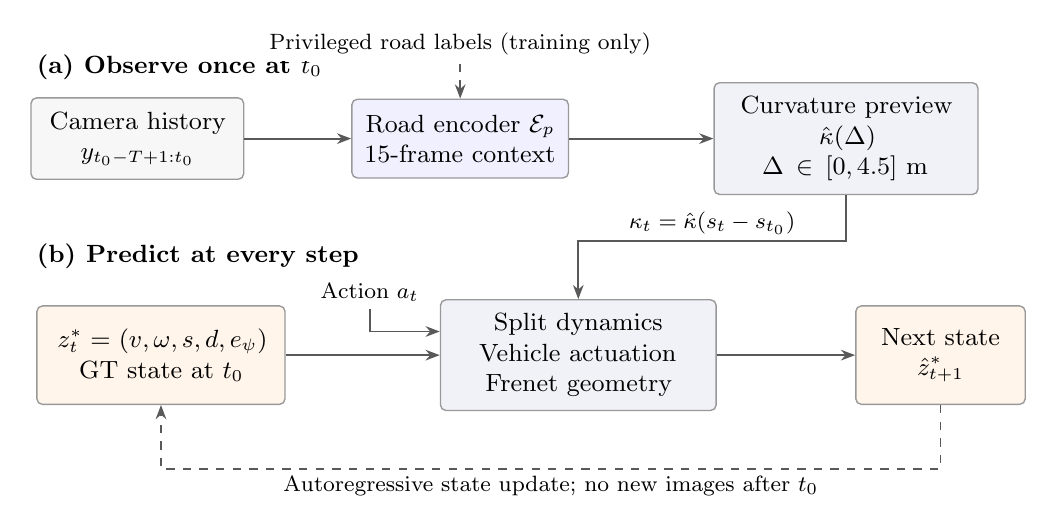
\begin{tikzpicture}[x=1cm,y=1cm,font=\fontsize{9}{11}\selectfont,
 box/.style={draw=black!40,rounded corners=2pt,line width=.5pt,align=center,inner sep=5pt},
 ar/.style={-{Stealth[length=1.8mm]},line width=.7pt,draw=black!65},
 lab/.style={font=\fontsize{8}{10}\selectfont,fill=white,inner sep=2pt}]
\node[anchor=west,font=\bfseries\fontsize{9}{11}\selectfont] at (0,4.05) {(a) Observe once at $t_0$};
\node[box,fill=black!3,text width=2.35cm,minimum height=1cm] (cam) at (1.4,3.15)
 {Camera history\\$y_{t_0-T+1:t_0}$};
\node[box,fill=blue!6,text width=2.4cm,minimum height=1cm] (enc) at (5.5,3.15)
 {Road encoder $\mathcal E_p$\\15-frame context};
\node[box,fill=frenetink!7,text width=3cm,minimum height=1cm] (preview) at (10.4,3.15)
 {Curvature preview\\$\hat\kappa(\Delta)$\\$\Delta\in[0,4.5]$ m};
\draw[ar] (cam) -- (enc);
\draw[ar] (enc) -- (preview);
\node[lab,anchor=south] at (5.5,4.13) {Privileged road labels (training only)};
\draw[ar,dashed] (5.5,4.1) -- (enc.north);
\node[anchor=west,font=\bfseries\fontsize{9}{11}\selectfont] at (0,1.65) {(b) Predict at every step};
\node[box,fill=orange!8,text width=2.8cm,minimum height=1.25cm] (state) at (1.7,.4)
 {$z_t^*=(v,\omega,s,d,e_\psi)$\\GT state at $t_0$};
\node[box,fill=frenetink!7,text width=3.15cm,minimum height=1.25cm] (dyn) at (7.0,.4)
 {Split dynamics\\Vehicle actuation\\Frenet geometry};
\node[box,fill=orange!8,text width=1.8cm,minimum height=1.25cm] (next) at (11.6,.4)
 {Next state\\$\hat z^*_{t+1}$};
\draw[ar] (state) -- (dyn);
\draw[ar] (dyn) -- (next);
\draw[ar] (preview.south) -- (10.4,1.85) -- node[lab,above] {$\kappa_t=\hat\kappa(s_t-s_{t_0})$} (7,1.85) -- (dyn.north);
\node[lab] at (4.35,1.2) {Action $a_t$};
\draw[ar] (4.35,.98) |- ([yshift=3mm]dyn.west);
\draw[ar,dashed] (next.south) -- (11.6,-1.05) -- node[lab,below] {Autoregressive state update; no new images after $t_0$} (1.7,-1.05) -- (state.south);
\end{tikzpicture}
\caption{PIWM-Frenet computation used in the driving evaluation. (a) The camera
history supplies a curvature preview once per rollout; road labels supervise
this encoder only during training. (b) The current state, action and indexed
curvature drive the structured transition. Predictions are fed back, while the
preview remains fixed. The reported rollouts use ground-truth initialization;
the figure separates this state input from the camera-derived road preview.}
\label{fig:arch}
\end{figure}

\subsection{Learning Interpretable Representations}\label{sec:repr_learning}

The autoencoder maps high-dimensional observations to a physically interpretable
latent state aligned with the true physical state.
We follow the conference paper in considering two architectural approaches.

\paragraph{Intrinsic encoding}
The encoder $\mathcal{E}: Y \rightarrow Z^*$ maps an observation directly to the
interpretable latent, partitioned as $\zstar = [z_p^*, z_{\mathrm{app}}^*]$, where
$z_p^*$ is the physically interpretable component and $z_{\mathrm{app}}^*$ captures
the residual appearance information needed for reconstruction. The conference
version writes the latter $z_v^*$; we rename it here because this article uses the
superscript $v$ for the \emph{vehicle} component of the factorized state.
For continuous latent spaces, the objective follows a $\beta$-VAE formulation with
interpretability alignment applied to $z_p^*$:
\begin{equation}
\mathcal{L}_{\mathrm{intrinsic\text{-}cont}} =
    \mathcal{L}_{\mathrm{recon}}(y, \hat{y})
    + \lambda_{\mathrm{interp}}\,\mathcal{L}_{\mathrm{interp}}(z_p^*, \Xi)
    + \beta\, D_{\mathrm{KL}}\!\left(q(z_{\mathrm{app}}^*|y)\,\|\,\mathcal{N}(0,I)\right).
\end{equation}
For discrete latent spaces, the codebook is partitioned so that each entry
$\mathbf{e}_k = [\mathbf{e}_k^p, \mathbf{e}_k^v]$ has a fixed physical component
and a learnable visual component.
The interpretability loss is applied to the averaged physical part of the
selected codebook entries.

\paragraph{Extrinsic encoding}
The extrinsic approach decouples visual perception from physical interpretation
via a two-stage process.
In the first stage, a vision autoencoder $(\mathcal{E}_v, \mathcal{D}_v)$ is
trained on image reconstruction only, producing an intermediate latent
$z = \mathcal{E}_v(y)$.
For continuous variants this is a $\beta$-VAE; for discrete variants a VQ-VAE
with a 512-entry codebook.
In the second stage, the vision encoder is frozen and a physical encoder
$\mathcal{E}_p$, paired with a physical decoder $\mathcal{D}_p$ that maps the
interpretable state back to the intermediate latent, is trained to produce
$\zstar = \mathcal{E}_p(z)$, optimizing:
\begin{equation}
    \mathcal{L}_{\mathrm{physical}} =
    \lambda_{\mathrm{interp}}\,\mathcal{L}_{\mathrm{interp}}(\zstar, \Xi)
    + \lambda_{\mathrm{latent}}\,\mathcal{L}_{\mathrm{recon}}\!\left(z,
    \mathcal{D}_p(\zstar)\right).
\end{equation}
The physical encoder $\mathcal{E}_p$ maps the temporal latent sequence to the
factorized state $\zstar = [\zv, \zr]$ (Section~\ref{sec:encoding}).

\paragraph{Which encoder for driving}
The conference paper's systematic comparison found that the extrinsic approach
with a discrete (VQ) latent gave the strongest physical grounding and prediction
accuracy, and it would be natural to carry that configuration over here.
We do not, and the reason is worth stating rather than glossing: that comparison
was run on \emph{fully observable} benchmarks, where the quantity to be encoded is
the controlled body's own state and a single frame nearly determines it.
The road-context encoder faces a different problem---reading the geometry of the
scene ahead out of a short, partially informative image window---so the conference
ranking is an extrapolation, not a result.
We therefore tested it directly, implementing the claimed configuration (per-frame
convolutional encoder, a $512$-entry VQ bottleneck, and a Transformer with
self-attention over the temporal window) at matched capacity and training it to
convergence on the same data as the encoder we ship.
It is worse at the perception task ($\mathrm{RMSE}_\kappa$ \SI{0.219}{} against
\SI{0.154}{m^{-1}}) and indistinguishable downstream: paired within folds, its
100-step position error differs from the shipped encoder's by less than a
millimeter (Table~\ref{tab:kappa_source}).
The driving experiments therefore use a convolutional encoder over the stacked
window with a linear curvature head, trained from scratch on the road-context
objective; the VQ--Transformer variant is reported as a baseline.
Section~\ref{sec:donkeyreal_results} returns to why the two differ so much less
downstream than they do at perception.

\paragraph{Interpretability loss}
For all variants, alignment between the encoded state and the physical variables
is enforced through the mean squared error to the empirical mean of the
supervisory samples:
\begin{equation}
    \mathcal{L}_{\mathrm{interp}}(\zstar, \Xi)
    = \left\| \zstar - \hat{\mu}_\Xi \right\|_2^2,
    \quad \hat{\mu}_\Xi = \frac{1}{L}\sum_{l=1}^L \xi^{(l)}.
    \label{eq:interp_loss}
\end{equation}
When applied to the factorized state, this loss is evaluated separately on the
vehicle-relative and road-context components with supervision from $\Xi^v$ and
$\Xi^r$:
\begin{equation}
    \mathcal{L}_{\mathrm{interp}}^{\mathrm{drive}} =
    \lambda_v\,\mathcal{L}_{\mathrm{interp}}(\zv, \Xi^v)
    + \lambda_r\,\mathcal{L}_{\mathrm{interp}}(\zr, \Xi^r).
    \label{eq:interp_loss_drive}
\end{equation}
The separate weighting of the road-context term $\lambda_r$ is what forces the
encoder to commit capacity to the external environment rather than only to the
vehicle.

%% --------------------------------------------------------------
\subsection{Encoding the Road Environment}\label{sec:encoding}  %% [NEW]
%% --------------------------------------------------------------

\paragraph{Challenge and motivation}
The conference model encoded only the controlled body's state, which for the
benchmarks was directly inferable from a single frame.
Road context is different in two ways.
First, it is a property of the \emph{environment}, not the agent, so it must be
read off the scene rather than the vehicle's appearance.
Second, for a forward-facing camera it is only \emph{partially visible}: at any
instant the camera sees a limited stretch of road, and quantities such as the
curvature of the lane the vehicle is about to enter are not fully determined by
the current frame.
A single-frame encoder is therefore insufficient; the road context must be
aggregated over time.

\paragraph{Temporal road-context encoder}
We condition the physical encoder on a history of visual latents:
\begin{equation}
    (\zv_t,\; \zr_t) = \mathcal{E}_p(z_{t-k+1:t}),
    \qquad z_{\tau} = \mathcal{E}_v(y_{\tau}),
    \label{eq:temporal_encoder}
\end{equation}
where $k$ is the context-window length.
Conditioning on a window rather than a frame is what makes the road context
identifiable: as the vehicle advances, geometry that was previously seen far ahead
becomes the geometry the vehicle is on, so the window supplies the parallax and
motion cues that disambiguate cross-track error, heading error and curvature,
which a single frame leaves ambiguous.
In practice we realize $\mathcal{E}_p$ convolutionally, with the $k$ frames of the
window entered as input channels and a linear curvature head on the pooled
features; a self-attention alternative over the same window was evaluated and did
not help (Table~\ref{tab:kappa_source}).
The encoder produces both components jointly but supervises them separately
through~\eqref{eq:interp_loss_drive}, ensuring $\zr_t$ carries genuine
environmental information rather than being absorbed into the vehicle component.

\paragraph{Privileged supervision for real-world deployment}
On the real DonkeyCar, the road context cannot be measured by the deployed car
itself.
We therefore use \emph{privileged supervision}: during training, an external
localization system (a known track map together with the logged car pose, as is
also obtainable from an overhead camera) provides ground-truth road context
$\Xi^r$ for each frame; at test time this signal is withheld and the deployed car
observes only its front camera.
The encoder~\eqref{eq:temporal_encoder} is thus trained to predict, from the
onboard image stream alone, the road context that the privileged signal supplied
during training.
This is precisely a teacher--student / learning-from-privileged-information
setup~\cite{chen2020learning}.
Because $\zr$ is physically interpretable, the recovered road context can be
inspected and compared against the true lane geometry, which we use as a
diagnostic in Section~\ref{sec:results}.

\begin{figure}[t]
\centering
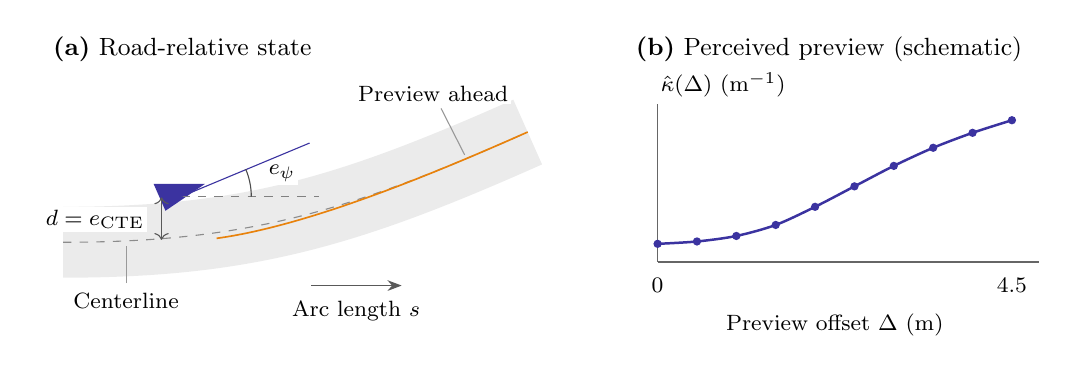
\begin{tikzpicture}[x=1cm,y=1cm,font=\fontsize{9}{11}\selectfont,
 ar/.style={-{Stealth[length=1.8mm]},draw=black!65,line width=.6pt},
 lab/.style={font=\fontsize{8}{10}\selectfont,fill=white,inner sep=1pt}]
\node[anchor=west] at (0,3.35) {\textbf{(a)} Road-relative state};
\node[anchor=west] at (7.4,3.35) {\textbf{(b)} Perceived preview (schematic)};
\draw[line width=9mm,black!8] (.25,.9) .. controls (2.6,.9) and (3.9,1.3) .. (6.15,2.3);
\draw[black!45,dashed] (.25,.9) .. controls (2.6,.9) and (3.9,1.3) .. (6.15,2.3);
\draw[line width=.6pt,previewor] (2.2,.95) .. controls (3.3,1.1) and (4.8,1.7) .. (6.15,2.3);
\fill[frenetink] (2.05,1.64) -- (1.4,1.64) -- (1.55,1.3) -- cycle;
\draw[<->,black!65] (1.5,.93) -- (1.5,1.47);
\node[lab,anchor=east] at (1.32,1.19) {$d=e_{\mathrm{CTE}}$};
\draw[black!50,dashed] (1.75,1.48) -- (3.5,1.48);
\draw[frenetink] (1.75,1.48) -- (3.38,2.16);
\draw[black!70] (2.64,1.48) arc (0:23:0.89);
\node[lab] at (3.03,1.77) {$e_\psi$};
\draw[ar] (3.4,.35) -- (4.55,.35);
\node[lab,anchor=north] at (3.97,.2) {Arc length $s$};
\node[lab,anchor=north] at (1.05,.3) {Centerline};
\draw[black!40] (1.05,.38) -- (1.05,.85);
\node[lab,anchor=south] at (4.95,2.65) {Preview ahead};
\draw[black!40] (5.05,2.6) -- (5.35,2.01);
\draw[black!60] (7.8,.65) -- (12.65,.65);
\draw[black!60] (7.8,.65) -- (7.8,2.65);
\node[lab,anchor=south west] at (7.8,2.7) {$\hat\kappa(\Delta)$ ($\mathrm{m}^{-1}$)};
\node[lab,anchor=north] at (7.8,.48) {$0$};
\node[lab,anchor=north] at (12.3,.48) {$4.5$};
\node[lab,anchor=north] at (10.05,.03) {Preview offset $\Delta$ (m)};
\draw[frenetink,line width=.9pt] plot[smooth] coordinates {(7.8,.88)(8.3,.91)(8.8,.98)(9.3,1.12)(9.8,1.35)(10.3,1.61)(10.8,1.87)(11.3,2.1)(11.8,2.29)(12.3,2.45)};
\foreach \x/\y in {7.8/.88,8.3/.91,8.8/.98,9.3/1.12,9.8/1.35,10.3/1.61,10.8/1.87,11.3/2.1,11.8/2.29,12.3/2.45}
 {\fill[frenetink] (\x,\y) circle (1.5pt);}
\end{tikzpicture}
\caption{Road state and camera-derived context. (a) The road-relative state is
$z^r=(s,e_{\mathrm{CTE}},e_\psi)$: progress along the centerline, signed lateral
offset and heading relative to the road tangent. (b) The encoder supplies ten
curvature samples over a \SI{4.5}{m} preview. This schematic profile is separate
from the propagated state and is held fixed during rollout.}
\label{fig:encoding}
\end{figure}

%% --------------------------------------------------------------
\subsection{Predicting the Road Environment}\label{sec:prediction}  %% [NEW]
%% --------------------------------------------------------------

\paragraph{Challenge and motivation}
Encoding the road at the current step is necessary but not sufficient.
To roll out a trajectory over a long horizon without new observations, the world
model must anticipate how the road context itself changes as the vehicle advances:
the curve that is ahead now is underfoot a few steps later, and the cross-track
and heading errors evolve as the vehicle tracks (or departs from) the lane.
A model that predicts only the vehicle state, holding the road context fixed or
ignoring it, drifts quickly because it steers the predicted vehicle through a road
that no longer matches reality.
We therefore make road prediction an explicit, physically interpretable part of
the dynamics.

\paragraph{Split dynamics}
We use a \emph{split-dynamics} model that advances the vehicle and the road
context with separate, physically appropriate transitions:
\begin{align}
    \hat{\zv}_{t+1} &= \phi^{v}_\theta(\zv_t,\; a_t),
        \label{eq:split_vehicle}\\
    \hat{\zr}_{t+1} &= f_r(\zr_t,\; \zv_t;\; \theta_r).
        \label{eq:split_road}
\end{align}
The vehicle transition $\phi^{v}_\theta$ is a structured kinematic model with a
small learned actuation map (below); the road transition $f_r$ is a geometry-driven
model (below). The superscript distinguishes it from the conference version's
$\phi$, which advances the whole state from two previous steps; here only the
vehicle branch is advanced, and from one.
Note which arguments $f_r$ does and does not take.
It consumes the vehicle's \emph{motion}---which over a rollout is the model's
own prediction from the preceding step---and not the action: the road context
is advected by how far and how the vehicle moved, so an action influences the
road only through the motion it produces.
(The one exception is the small bounded residual in
\eqref{eq:frenet_d}--\eqref{eq:frenet_psi}, which is conditioned on the
action.)
This is what makes the second equation a transport rule rather than a second
learned dynamics model.
Splitting the dynamics decouples the fast-varying vehicle motion from the
slow-varying road geometry and lets each receive its correct inductive bias.

\paragraph{Structured kinematics for the vehicle}
For driving environments we replace the generic second-order dynamics of the
conference paper with a wheeled-vehicle kinematic prior.
In the body frame this is the classical \emph{bicycle kinematic model}
\begin{align}
    x_{t+1}    &= x_t    + v_t\cos(\psi_t + \beta_t)\,\Delta t,
    \label{eq:bic_x}\\
    y_{t+1}    &= y_t    + v_t\sin(\psi_t + \beta_t)\,\Delta t,
    \label{eq:bic_y}\\
    \psi_{t+1} &= \psi_t + \frac{v_t}{l_r}\sin(\beta_t)\,\Delta t,
    \label{eq:bic_psi}
\end{align}
with slip angle
$\beta_t = \arctan\!\left(\frac{l_r}{l_f + l_r}\tan(\delta_{f,t})\right)$, where
$l_f$ and $l_r$ are the distances from the center of mass to the front and rear
axles (unknown and learned during training), $\delta_{f,t}$ is the steering
angle, $v_t$ the longitudinal speed and $\psi_t$ the heading.

Because the road context is itself defined relative to the lane
(Section~\ref{sec:factorized_state}), we express the vehicle in the same
road-aligned frame, which yields the equivalent kinematics
\eqref{eq:frenet_s}--\eqref{eq:frenet_psi} below and lets the two branches of the
split dynamics share one geometry.
In either frame the \emph{pose} kinematics are analytic; what is unknown is how
the commanded action drives the vehicle.
We therefore learn only a compact actuation map
\begin{equation}
    v_{t+1} = v_t + g^v_\theta(\zv_t, \zr_t, a_t),
    \qquad
    \omega_{t+1} = \omega_t + g^\omega_\theta(\zv_t, \zr_t, a_t),
    \label{eq:actuation}
\end{equation}
where $g^v_\theta$ and $g^\omega_\theta$ are small multilayer perceptrons mapping
throttle to longitudinal acceleration and steering to yaw acceleration.
Every remaining quantity in the vehicle branch is a physical variable propagated
by an analytic equation.

\paragraph{Structured road-context transition}
The road-context state $(e_{\mathrm{CTE}}, e_\psi, \kappa)$ evolves slowly and
geometrically.
As the vehicle moves by the increment implied by its predicted motion, the road
ahead is effectively re-indexed: the lane geometry is advected past the vehicle.
We therefore model $f_r$ as a geometry-driven transition that (i) updates the
cross-track and heading errors from the vehicle's predicted lateral and angular
motion relative to the road, and (ii) does \emph{not} integrate the curvature
forward at all, but re-reads it from the already-perceived preview at the arc
length the vehicle has covered.

Concretely, we work in a road-aligned (Frenet) frame in which the vehicle state
is $(s, e_{\mathrm{CTE}}, e_\psi, v, \omega)$, with $s$ the arc length along the
lane center, $v$ the longitudinal speed and $\omega$ the yaw rate.
Writing $\kappa_t = \hat{\kappa}(s_t)$ for the perceived curvature at the current
arc length and $\eta_t = 1 - e_{\mathrm{CTE},t}\kappa_t$ for the Jacobian of the
road-aligned parameterization, the transition is
\begin{align}
    s_{t+1} &= s_t + \frac{v_t\cos e_{\psi,t}}{\eta_t}\,\Delta t,
        \label{eq:frenet_s}\\
    e_{\mathrm{CTE},t+1} &= e_{\mathrm{CTE},t}
        + v_t \sin e_{\psi,t}\,\Delta t + \varepsilon^d_{\theta_r},
        \label{eq:frenet_d}\\
    e_{\psi,t+1} &= e_{\psi,t}
        + \Bigl(\omega_t - \kappa_t\,\frac{v_t\cos e_{\psi,t}}{\eta_t}\Bigr)\Delta t
        + \varepsilon^\psi_{\theta_r},
        \label{eq:frenet_psi}\\
    \kappa_{t+1} &= \hat{\kappa}(s_{t+1}),
        \label{eq:frenet_kappa}
\end{align}
where $\Delta t$ is the sampling interval and
$(\varepsilon^d_{\theta_r}, \varepsilon^\psi_{\theta_r})$ is a small learned
residual, tightly bounded, that corrects effects the rigid geometric update
misses (e.g., imperfect lane tracking).
Equations~\eqref{eq:frenet_s}--\eqref{eq:frenet_psi} are analytic; only the
residual and the actuation map~\eqref{eq:actuation} are learned.

Equation~\eqref{eq:frenet_kappa} is the crucial one.
The curvature is a \emph{lookup into the curvature profile already perceived at
the start of the rollout} (Section~\ref{sec:encoding}), indexed by how far the
predicted vehicle has traveled.
It is therefore not a free latent that the dynamics must propagate, and it cannot
accumulate error over the horizon: the road is \emph{observed} once and then
re-indexed, not extrapolated.
This is the structural reason the rollout stays bounded, and it is what
distinguishes the model from world models that carry the road as an unconstrained
latent that drifts and, in turn, corrupts the vehicle branch that consumes it.
The preview is long enough for this to be well defined for most of the horizon:
over a 100-step rollout the vehicle covers on average \SI{3.1}{m} of arc length,
staying inside the \SI{4.5}{m} perceived preview in $82\%$ of evaluation windows;
past the preview the model holds the last perceived value rather than
extrapolating.
Because $f_r$ operates on the physically interpretable $\zr$, the forecasted road
context at any horizon is itself interpretable: the model outputs a predicted
lane geometry that can be visualized and checked, not an opaque feature.

\begin{figure}[t]
\centering
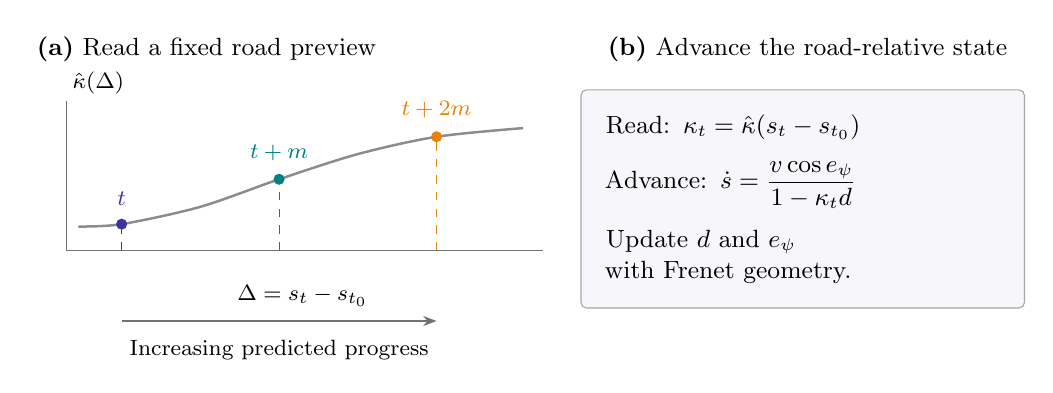
\begin{tikzpicture}[x=1cm,y=1cm,font=\fontsize{9}{11}\selectfont,
 ar/.style={-{Stealth[length=1.7mm]},line width=.65pt},
 lab/.style={font=\fontsize{8}{10}\selectfont,fill=white,inner sep=2pt}]
\node[anchor=west] at (0,3.8) {\textbf{(a)} Read a fixed road preview};
\node[anchor=west] at (7.25,3.8) {\textbf{(b)} Advance the road-relative state};
\draw[black!55] (.5,1.25) -- (6.55,1.25);
\draw[black!55] (.5,1.25) -- (.5,3.15);
\node[lab,anchor=south west] at (.5,3.15) {$\hat\kappa(\Delta)$};
\node[lab,anchor=north] at (3.5,.88) {$\Delta=s_t-s_{t_0}$};
\draw[black!45,line width=.9pt] plot[smooth] coordinates {(.65,1.55)(1.2,1.58)(2.2,1.8)(3.2,2.15)(4.2,2.47)(5.2,2.69)(6.3,2.8)};
\foreach \x/\y/\c/\t in {1.2/1.58/frenetink/t,3.2/2.15/teal/t+m,5.2/2.69/previewor/t+2m} {
 \draw[\c,dashed] (\x,1.25) -- (\x,\y);
 \fill[\c] (\x,\y) circle (2pt);
 \node[lab,anchor=south,text=\c] at (\x,\y+.16) {$\t$};}
\draw[ar,black!55] (1.2,.35) -- (5.2,.35);
\node[lab,anchor=north] at (3.2,.19) {Increasing predicted progress};
\node[draw=black!35,rounded corners=2pt,fill=frenetink!4,align=left,
 text width=5.0cm,inner sep=9pt] at (9.85,1.9) {
 Read: $\kappa_t=\hat\kappa(s_t-s_{t_0})$\\[7pt]
 Advance: $\dot s=\dfrac{v\cos e_\psi}{1-\kappa_t d}$\\[7pt]
 Update $d$ and $e_\psi$\\with Frenet geometry.};
\end{tikzpicture}
\caption{Road prediction by re-indexing. (a) Successive states query the same
camera-derived curvature profile at increasing arc-length offsets. (b) Frenet
kinematics advance progress, lateral offset and heading error, with the learned
corrections described in the text. The profile itself is not extrapolated;
perception and state-integration errors can still affect the rollout.}
\label{fig:prediction}
\end{figure}

\subsection{Training Procedure}

Training follows a staged pipeline.
Stage~1 trains the vision autoencoder $(\mathcal{E}_v, \mathcal{D}_v)$ on image
reconstruction.
Stage~2 trains the physical encoder $\mathcal{E}_p$ to produce the factorized
interpretable state, optimizing~\eqref{eq:interp_loss_drive} jointly with a latent
reconstruction term.
Stage~3 trains the split-dynamics models ($\phi^{v}_\theta$ for the vehicle and $f_r$
for the road context), with an optional end-to-end fine-tuning pass that updates
the encoder and dynamics together to align the encoded state with what the
dynamics can predict.
Algorithm~\ref{alg:piwm_drive} summarizes the procedure.

\begin{algorithm}[p]
\caption{PIWM training for partially observable driving.}
\label{alg:piwm_drive}
\begin{algorithmic}[1]
\Require Training set $\mathcal{S}$, loss weights
         $\lambda_v, \lambda_r, \lambda_{\mathrm{latent}}$, context length $k$
\State Train vision autoencoder $(\mathcal{E}_v, \mathcal{D}_v)$ on image
       reconstruction
\For{each batch $(y_{1:M}, a_{1:M}, \Xi^v_{1:M}, \Xi^r_{1:M})$}
    \State $z_t \gets \mathcal{E}_v(y_t)$ for all $t$
    \State $(\zv_t, \zr_t) \gets \mathcal{E}_p(z_{t-k+1:t})$
           \Comment{encode vehicle and road (Sec.~\ref{sec:encoding})}
    \State Update $\mathcal{E}_p$ with
           $\lambda_v\,\mathcal{L}_{\mathrm{interp}}(\zv_t, \Xi^v_t)
           + \lambda_r\,\mathcal{L}_{\mathrm{interp}}(\zr_t, \Xi^r_t)
           + \lambda_{\mathrm{latent}}\,\mathcal{L}_{\mathrm{recon}}$
\EndFor
\For{each batch}
    \State Obtain $(\zv_t, \zr_t)$ from the encoders
    \State $\hat{\zv}_{t+1} \gets \phi^{v}_\theta(\zv_t, a_t)$
           \Comment{bicycle model}
    \State $\hat{\zr}_{t+1} \gets f_r(\zr_t, \zv_t;\,\theta_r)$
           \Comment{road prediction (Sec.~\ref{sec:prediction})}
    \State Update $\theta$ (bicycle) and $\theta_r$ (road) on the multi-step
           rollout loss
           $\|\hat{\zv}_{t+1} - \hat{\mu}_{\Xi^v_{t+1}}\|^2
           + \|\hat{\zr}_{t+1} - \hat{\mu}_{\Xi^r_{t+1}}\|^2$
\EndFor
\State (Optional) End-to-end fine-tune $\mathcal{E}_p, \phi^{v}_\theta, f_r$ jointly
\State \Return trained model parameters
\end{algorithmic}
\end{algorithm}


%% ==============================================================
\section{Experimental Evaluation}\label{sec:experiments}
%% ==============================================================

\subsection{Environments and Evaluation Tiers}

We evaluate across three tiers of increasing difficulty.
Tier~1 establishes continuity with the conference paper; Tiers~2 and~3 are the two
new partially observable driving case studies (Contribution~1).

\paragraph{Tier~1: Conference benchmarks}
The conference evaluation~\cite{piwm_conf} comprises \textbf{CartPole},
\textbf{Lunar Lander}~\cite{brockman2016openai}, and the \textbf{DonkeyCar
simulator}. CartPole and Lunar Lander provide controlled physical systems; the
simulator provides a visual driving benchmark with an approximate bicycle prior.
Figure~\ref{fig:conf_environments} shows their original observations. We retain
these experiments to document the original representation-learning results,
separately from the new road-context evaluation on the physical DonkeyCar.

\begin{figure}[t]
\centering
\includegraphics[width=\linewidth]{fig_conference_environments.pdf}
\caption{Original conference environments: CartPole, Lunar Lander and the
DonkeyCar simulator. Frames are extracted from the ground-truth rows of the
conference qualitative figures~\cite{piwm_conf}; the simulated driving scene
is distinct from the physical platform evaluated in Tier~3.}
\label{fig:conf_environments}
\end{figure}

\paragraph{Tier~2: Partially observable simulated driving (CarRacing)}
\textbf{CarRacing}, from the OpenAI Gym suite~\cite{brockman2016openai}, is a
top-down simulated racing environment in which the vehicle navigates a
procedurally generated track.
Its observation is a bird's-eye-view RGB image, $96 \times 96$ as the environment
returns it, which we resize to $64 \times 64$ for the encoder.
The vehicle's kinematic state is available from the simulator, but the road
geometry (the shape of the upcoming track and the vehicle's relationship to the
lane) is not part of the state and must be inferred from the image.
Because the camera is top-down, the road ahead is visible but the model must still
\emph{encode} it into the physical road context and \emph{predict} its evolution
during rollout.
This is the controlled setting in which the factorized-state formulation and the
split dynamics were developed; the quantitative evaluation reported in this
article is on the physical platform of Tier~3, for the reason given in
Section~\ref{sec:carracing_results}.

\paragraph{Tier~3: Real-world DonkeyCar deployment}
The \textbf{DonkeyCar (real)} tier evaluates the factorized formulation on a
physical RC-scale autonomous car driven on a laboratory track.
The car observes its environment through a front-facing camera (the test-time
observation, $64 \times 64$), and logs wheel-encoder speed, steering, and pose.
This is the most demanding tier: the camera is forward-facing, so the road ahead
is only partially visible, and the road context cannot be measured by the deployed
car.
We collect driving trajectories on the physical platform and derive ground-truth
road context from external track localization, used as privileged supervision at
training time only (Section~\ref{sec:encoding}); at test time the model infers and
rolls out road context from the onboard front-camera stream alone.

\subsection{Experimental Setup}\label{sec:setup}

\paragraph{Benchmarks (Tier~1)}
The data-collection and weak-supervision protocol follows the conference paper.
The conference study collected 60{,}000 trajectories of at least 50 steps per environment,
generated by a mix of random actions and a pretrained neural controller.
Weak-supervision labels are synthesized by adding biased uniform noise of relative
width $\delta \in \{0\%, 5\%, 10\%\}$ to the ground-truth state, as described in
\ref{sec:interp_loss_def}.

\paragraph{CarRacing (Tier~2)}
Driving data are generated with a pretrained controller on procedurally generated
tracks; each episode records the onboard image, action, and simulator state.
Ground-truth labels for the vehicle pose and for the road context are available
directly from the simulator and its track geometry.
We use exact ground-truth labels for training (corresponding to $\delta = 0$) and
evaluate whether the factorized-state formulation improves long-horizon prediction
relative to baselines that use only vehicle-state labels.

\paragraph{DonkeyCar real (Tier~3)}
We drive the physical DonkeyCar on a closed laboratory track and record
synchronized front-camera frames ($64 \times 64$), control actions
(steering, throttle), and vehicle pose, at approximately \SI{22}{fps}, so that
$\Delta t = 1/22\,\mathrm{s}$ and the 100-step evaluation horizon corresponds to
about \SI{4.5}{s} of driving.
Trajectories are segmented into clean contiguous laps; brief sensing artifacts
(dropped or interpolated frames, pose glitches) are filtered out before training.
Ground-truth road context is computed from the known track centerline and the
logged pose (privileged supervision), and is withheld at test time.
The main comparison uses five folds over 71 episodes, totaling 2{,}483
validation windows; each fold holds out disjoint episodes. Position errors are
reported in meters. The legacy 201-window split is used only where explicitly
identified.

\paragraph{Architecture and training}
The driving experiments use a vision encoder followed by a physical head that
produces the factorized state. The head is trained directly against the road-context
labels rather than through a reconstruction objective, because road context is
available under privileged supervision at training time and nothing has to be
learned by reconstructing the image. This is a departure from the conference
version's autoencoding variants, so we implemented those as well and measured them
here rather than inheriting their ranking (Table~\ref{tab:kappa_source}); on this
task the choice does not move the rollout error.
The vision encoder maps each $64 \times 64$ observation to a compact latent, and
the physical encoder aggregates a context window of $T_{\mathrm{ctx}} = 15$ frames
($\approx$\SI{0.7}{s}) to infer the road context from image sequences
(Section~\ref{sec:encoding}).
Our rollouts are trained on $16$-step horizons and evaluated at up to $100$ steps,
so the reported horizon is more than six times the training horizon; the baselines
are trained on $32$-step rollouts, i.e.\ twice ours, which if anything favors
them at the horizons where we claim an advantage.
Dynamics are trained with Adam, a cosine learning-rate schedule and early stopping
on validation loss.
All baselines are trained under identical conditions with the same data, the same
optimizer and the same evaluation protocol, and with the batch sizes at which each
baseline was tuned; we verified that increasing the batch size degrades these
small, latency-bound baselines and would therefore have flattered our model.

\subsection{Baselines}\label{sec:baselines}

We compare against the same families used in the conference paper.
\textbf{DVBF}~\cite{karl2016deep} is a latent state-space model with a
locally-linear transition and no physical prior; \textbf{GOKU-net}
~\cite{linial_generative_2021} and \textbf{Vid2Param}~\cite{asenov2019vid2param}
are physics-aware, the first constraining its latent to a known ODE and the second
inferring the parameters of a known analytic model; and
\textbf{SINDYc}~\cite{BRUNTON2016710} is a classical dynamics-discovery baseline
operating on the interpretable latent.
Every baseline is initialized from the ground-truth vehicle state \emph{and} the
ground-truth lane waypoints at the first timestep of the window, so each starts
from an explicit description of the road that our model has to recover from
pixels.
They are then run as latent transition models, consuming only actions over the
rollout.
One asymmetry among them should be stated plainly, because it determines their
ordering.
Vid2Param additionally infers a latent parameter vector from the image window,
since inferring physical parameters from video is the whole of that method; it is
consequently the only baseline with any visual input, and it is also the strongest
one we measure.
DVBF and GOKU-net are run without their own observation pathways---DVBF without
its filtering step and GOKU-net without its inference of ODE parameters from the
observation sequence---so their numbers should be read as characterizing a
\emph{dynamics-only} version of each method rather than the method as published.
That reduction was made to hold the comparison at the level of the transition
model, but it is a limitation of our evaluation, not a property of those methods,
and the gap between our model and them is correspondingly easier to obtain than
the gap against Vid2Param.
To separate the contribution of \emph{perceiving} the road from that of
\emph{representing} it, we also evaluate a privileged \textbf{oracle} variant of
our own model in which $\kappa$ is read from the known track map instead of the
camera; the gap between the two is the cost of perception.

\subsection{Metrics}

The primary driving metric is the \emph{position error at rollout step $k$}: the
Euclidean distance, in meters, between the predicted and the true vehicle
position after $k$ autoregressive steps, averaged over the $N = 201$ held-out
validation windows,
\begin{equation}
    E_{xy}(k) = \frac{1}{N}\sum_{i=1}^{N}
    \bigl\lVert \hat{p}_{i,k} - p_{i,k} \bigr\rVert_2 ,
    \qquad
    \label{eq:metric_exy}
\end{equation}
where $p_{i,k}$ is the ground-plane position of the vehicle at rollout step $k$ of
window $i$, in meters, and $\hat{p}_{i,k}$ the model's prediction of it. All models
are compared in the same planar frame, whatever internal parameterization each
uses.
We report $E_{xy}$ at $k \in \{25, 50, 100\}$ and plot the full curve
$k \mapsto E_{xy}(k)$; all rollouts are initialized from the ground-truth state at
$k=0$ so that the comparison isolates the dynamics rather than the encoder.
Because $E_{xy}$ is a distance and not a squared error, its values are directly
readable as centimeters of drift.
We additionally report the curvature error of the road-context encoder,
$\mathrm{RMSE}_\kappa$ in $\mathrm{m}^{-1}$, to evaluate the encoded road
directly.
For benchmark tasks (Tier~1) we follow the conference protocol and report state
RMSE over all state dimensions at a 30-step horizon, together with the relative
parameter-recovery error for the environments whose ground-truth physical
parameters are known (CartPole, Lunar Lander).


%% ==============================================================
\section{Results}\label{sec:results}
%% ==============================================================

\subsection{Conference Benchmark Results (Tier~1)}\label{sec:conf_results}

We restore the original conference results~\cite{piwm_conf} in
Figures~\ref{fig:conf_cartpole}--\ref{fig:conf_rollouts}. These are inherited
experiments, not additional runs of PIWM-Frenet. They compare intrinsic and
extrinsic encoders with continuous or discrete latents over 30 prediction steps
and supervision-noise levels $\delta\in\{0,5\%,10\%\}$. The conference protocol
uses five-fold cross-validation. State RMSE in these benchmarks is distinct from
the meter-valued position error of the physical-car evaluation.

\paragraph{Prediction and architectural choice}
Figures~\ref{fig:conf_cartpole}, \ref{fig:conf_lunar} and
\ref{fig:conf_donkey} retain all six panels for each environment. Extrinsic
PIWM with discrete latents gives the lowest long-horizon error among the
extrinsic variants shown. The intrinsic setting has a different ranking:
continuous PIWM generally outperforms the discrete variant. Thus the conference
results support choosing the latent parameterization together with the encoder
architecture, rather than a universal advantage for quantization. The driving
encoder comparison in Table~\ref{tab:kappa_source} revisits this choice for the
new road-perception task.

\begin{figure}[p]
\centering
\includegraphics[width=\linewidth]{fig_conference_cartpole.pdf}
\caption{Conference CartPole results~\cite{piwm_conf}. State RMSE over 30 steps
for (a) extrinsic and (b) intrinsic methods, under three supervision-noise
levels. Curves and shaded regions are the original embedded plot images;
labels and layout have been reset. Panel-specific vertical limits are retained.
The archived figure does not specify the statistical meaning of its shading.}
\label{fig:conf_cartpole}
\end{figure}

\begin{figure}[p]
\centering
\includegraphics[width=\linewidth]{fig_conference_lunar.pdf}
\caption{Conference Lunar Lander results~\cite{piwm_conf}. The layout and
method groups follow Figure~\ref{fig:conf_cartpole}. Original curves and shaded
regions are preserved; all panels retain the source RMSE range $[0,2]$.}
\label{fig:conf_lunar}
\end{figure}

\begin{figure}[p]
\centering
\includegraphics[width=\linewidth]{fig_conference_donkey.pdf}
\caption{Conference DonkeyCar-simulator results~\cite{piwm_conf}. The layout
follows Figure~\ref{fig:conf_cartpole}. Original curves and shaded regions are
preserved, including the source vertical limit of 2; curves beyond that limit
are clipped as in the original. These are 30-step state-RMSE results and must
not be read as the 100-step position errors of the physical car.}
\label{fig:conf_donkey}
\end{figure}

\paragraph{Parameter estimates and visual rollouts}
Figure~\ref{fig:conf_parameters} restores the parameter comparison for CartPole
and Lunar Lander. The reference lines make both agreement and departures from
the known parameters visible as supervision noise changes. We omit the original
DonkeyCar wheelbase panel from this recovery comparison because it has no
known-parameter reference. Figure~\ref{fig:conf_rollouts} retains all five
comparison rows from the original visual rollout example, with three
display columns selected for legibility. These examples illustrate visual
behavior and do not replace the quantitative comparisons above. The original controller diagnostic is also
retained in Appendix~\ref{sec:conf_control}.

\begin{figure}[p]
\centering
\includegraphics[width=\linewidth]{fig_conference_parameters.pdf}
\caption{Conference parameter estimates for the two controlled
benchmarks~\cite{piwm_conf}. Each panel retains the original colored intervals,
center marks and yellow ground-truth reference. Rows correspond to
$\delta=0,5\%,10\%$, from top to bottom. Parameter names and scales follow the
source figure; the source does not specify the interval statistic.}
\label{fig:conf_parameters}
\end{figure}

\begin{figure}[p]
\centering
\includegraphics[width=\linewidth]{fig_conference_rollouts.pdf}
\caption{Conference visual rollouts at $\delta=5\%$~\cite{piwm_conf}.
Ground truth and the four original model rows are shown at $k=5,15,30$ for the
DonkeyCar simulator and Lunar Lander. Frames are extracted without retouching;
the intermediate display columns and the slide footer have been omitted.}
\label{fig:conf_rollouts}
\end{figure}
\FloatBarrier

\subsection{CarRacing (Tier~2)}\label{sec:carracing_results}

CarRacing serves in this article as the controlled simulated setting in which the
factorized formulation was developed: the road geometry is present in the image
but absent from the vehicle state, so the encoder must recover it from pixels
even though the top-down view makes the road ahead fully visible.
We do not report a quantitative baseline comparison for this tier here.
The comparison in an earlier version of this work was run with a vehicle-only
dynamics variant rather than the road-context model described in
Section~\ref{sec:prediction}, and re-running it with the present model is left to
future work; Section~\ref{sec:discussion} returns to this point.
All quantitative claims about the new road-context extension therefore rest on
the physical platform of Section~\ref{sec:donkeyreal_results}, where the forward-facing camera makes
partial observability genuine rather than nominal.

%% =================================================================
%% COMMENTED OUT --- DO NOT DELETE.
%% The CarRacing figure, table and analysis below are retained verbatim.
%% They were withdrawn because the row printed as "PIWM (ours, full)" was the
%% PIWM-bicycle-v4 column of _archive/logs/overnight.log, which is a
%% vehicle-only dynamic-bicycle model with NO road context, while the one
%% variant that did carry road context (PIWM-lane-v5, 0.0013/0.0333/0.2671/
%% 1.5950 at steps 20/50/75/100) was omitted from the table.  The numbers are
%% also MSE, not the RMSE declared in the Metrics subsection.
%% TO RESTORE: re-run the CarRacing comparison with the road-context model,
%% then uncomment, relabel the rows to match the checkpoints actually used,
%% state the metric explicitly, and re-check every claim in the analysis.
%% =================================================================
%% \subsection{CarRacing Results (Tier~2)}\label{sec:carracing_results_OLD}
%% 
%% \begin{figure*}[t]
%%     \centering
%%     \includegraphics[width=0.95\textwidth]{../vis/final_state_mse.png}
%%     \caption{Prediction performance on CarRacing. State error over a 100-step
%%     horizon for $x_{\mathrm{rel}}$, $y_{\mathrm{rel}}$, and $\psi_{\mathrm{rel}}$,
%%     comparing PIWM (with factorized state and split dynamics) against PIWM-linear,
%%     PIWM-bicycle (vehicle state only, no road context), SINDYc, GOKU-net, DVBF, and
%%     Vid2Param. Methods that encode and predict the road context remain accurate at
%%     long horizons, while vehicle-only and data-driven baselines diverge.}
%%     \label{fig:carracing}
%% \end{figure*}
%% 
%% Figure~\ref{fig:carracing} reports state error over a 100-step prediction horizon
%% on CarRacing.
%% Table~\ref{tab:carracing} summarizes the longitudinal-displacement
%% ($x_{\mathrm{rel}}$) error at representative horizons.
%% 
%% \begin{table}[t]
%% \centering
%% \caption{CarRacing longitudinal-displacement ($x_{\mathrm{rel}}$) prediction
%% error at increasing horizons (lower is better). PIWM with the bicycle model and
%% road-context factorization maintains low error to 100 steps, whereas the
%% vehicle-only ablations (PIWM-linear, PIWM-bicycle) and most baselines diverge.
%% \emph{The numerical entries are populated from our evaluation runs; confirm
%% against the final experiment freeze before submission.}}
%% \label{tab:carracing}
%% \small
%% \begin{tabular}{lrrrr}
%% \toprule
%% Model & step 20 & step 50 & step 75 & step 100 \\
%% \midrule
%% PIWM-linear            & 0.015 & 0.124 & 0.559 & 1.985 \\
%% PIWM-bicycle (veh.\ only) & 0.008 & 0.186 & 0.696 & 2.020 \\
%% SINDYc                 & 0.046 & 0.927 & 4.493 & 15.03 \\
%% DVBF                   & 0.009 & 0.182 & 1.242 & 3.556 \\
%% Vid2Param              & 0.001 & 0.094 & 1.093 & 6.044 \\
%% GOKU-net                & 0.001 & 0.038 & 0.324 & 1.405 \\
%% \textbf{PIWM (ours, full)} & \textbf{0.002} & \textbf{0.026} & \textbf{0.074} & \textbf{0.306} \\
%% \bottomrule
%% \end{tabular}
%% \end{table}
%% 
%% The proposed PIWM with the bicycle model and factorized state substantially
%% outperforms all baselines across the state dimensions and across the full 100-step
%% horizon.
%% Critically, the two ablations that drop the road context, PIWM-linear and
%% PIWM-bicycle (vehicle state only), are competitive at short horizons but diverge
%% as the horizon grows: by 75--100 steps their error is roughly an order of
%% magnitude larger than the full model.
%% This is the central empirical signature of partial observability.
%% A vehicle-only model cannot anticipate the upcoming road geometry, so once the
%% rollout enters curvature that was not represented, errors compound; the full
%% model, which encodes the road context and predicts its evolution, steers the
%% predicted vehicle through the correct geometry and stays accurate.
%% Data-driven baselines (LSTM-style and GOKU-net) and the physics-aware DVBF and
%% Vid2Param exhibit rapid error growth at long horizons, consistent with the
%% conference findings.
%% 
%% \paragraph{Quality of the predicted road environment}
%% Because $\zr$ is interpretable, we can inspect the forecasted road directly.
%% The predicted road context (cross-track error, heading error, curvature) tracks
%% the ground-truth lane geometry over the rollout, confirming that the model is not
%% merely improving vehicle prediction as a side effect but is genuinely forecasting
%% the external environment in physically meaningful terms.
%% 
\subsection{Real DonkeyCar Results (Tier~3)}\label{sec:donkeyreal_results}

We deploy the learned model on the physical DonkeyCar, where the road context is
supervised only during training and must be inferred from the front camera at
test time.
This is the setting the article is about: the camera sees a short stretch of road,
the vehicle state alone is non-Markov, and nothing about the track is available to
the deployed model beyond what it can read from its own images.

\paragraph{Long-horizon prediction against baselines}
Table~\ref{tab:donkey_main} and Figure~\ref{fig:donkey_main} report position error
over a 100-step ($\approx$\SI{4.5}{s}) autoregressive rollout under five-fold
cross-validation over the $71$ recorded episodes: each fold holds out one fifth of
them ($301$--$647$ evaluation windows, $2483$ in total), every model is trained on
that fold's training episodes only, and we average within a fold before reporting
the mean and standard deviation over the five fold-level means. Comparisons \emph{within} a
fold are paired---every model rolls out from the same initial states over the same
windows---and the paired statistics below are computed that way.
Two regimes are visible, and the crossover between them is the central result.
For the first two thirds of the horizon the physics-aware baselines are
\emph{ahead} of our model: Vid2Param in particular is nearly four times as accurate
at step $25$ (\SI{0.036}{m} against \SI{0.141}{m}).
This is expected, and it is a consequence of the comparison being generous to
them: each baseline is handed the ground-truth lane waypoints at $t_0$, so over
short horizons it is interpolating from a description of the road that our model
had to recover from pixels.
Beyond the crossover the ordering inverts and does not invert back: on the
fold-mean curves our model is ahead of DVBF from step $64$ onward, of GOKU-net from
step $75$ and of Vid2Param from step $82$.
By step $100$ it reaches \SI{0.463}{m} against \SI{0.703}{m} for the
strongest baseline. Within each fold, where the comparison is paired, our model is
ahead at step $100$ in \emph{all five} folds against every baseline: by
\SI{0.240}{m} on average against Vid2Param, \SI{0.262}{m} against GOKU-net and
\SI{0.374}{m} against DVBF.
SINDYc diverges in every one of the $2483$ evaluation windows of all five folds, so
we report it as divergent rather than quoting a value; past the point of divergence
the number records only where the rollout was clamped.

The more informative quantity is the spread. Changing which episodes are held out
moves our error by $\pm\SI{0.046}{m}$, against $\pm\SI{0.192}{m}$ for Vid2Param,
$\pm\SI{0.122}{m}$ for GOKU-net and $\pm\SI{0.160}{m}$ for DVBF---factors of
$2.7$ to $4.2$. The baselines' long-horizon error depends substantially on which part of
the track they were trained on; ours much less so. We regard this as the more
durable of the two claims, because it does not rest on any single trained model.

\begin{table}[t]
\centering
\caption{Position error $E_{xy}$ in meters on the physical DonkeyCar, at three
rollout horizons, as mean $\pm$ standard deviation over five-fold cross-validation (lower is
better). All models are driven by the same actions and are initialized from the
ground-truth state; the baselines additionally receive the ground-truth lane
waypoints at $t_0$. Of the baselines only Vid2Param also sees the images---DVBF
and GOKU-net are run as dynamics-only models (Section~\ref{sec:baselines}), which is
why Vid2Param leads them. Every model, ours included, keeps the epoch with the best
$E_{xy}(100)$; the last column also reports how much each model moves when the
held-out episodes change. The map-free row recovers position without consulting the
track map at all, reading the road geometry from the perception's shape output
instead of indexing a surveyed centerline.}
\label{tab:donkey_main}
\footnotesize
\setlength{\tabcolsep}{3.4pt}
\begin{tabular}{lrrr}
\toprule
Model & $E_{xy}(25)$ & $E_{xy}(50)$ & $E_{xy}(100)$ \\
\midrule
Vid2Param~\cite{asenov2019vid2param}   & $\mathbf{0.036 \pm 0.008}$ & $\mathbf{0.107 \pm 0.008}$ & $0.703 \pm 0.142$ \\
GOKU-net~\cite{linial_generative_2021}  & $0.046 \pm 0.012$ & $0.131 \pm 0.013$ & $0.725 \pm 0.107$ \\
DVBF~\cite{karl2016deep}               & $0.061 \pm 0.011$ & $0.173 \pm 0.031$ & $0.837 \pm 0.131$ \\
SINDYc~\cite{BRUNTON2016710}           & \multicolumn{3}{c}{diverges in all $2483$ windows of all five folds} \\
\midrule
\textbf{PIWM-Frenet (ours, perceived $\kappa$)} & $0.141 \pm 0.009$ & $0.245 \pm 0.021$ & $\mathbf{0.463 \pm 0.045}$ \\
\emph{PIWM-Frenet (map-free)} & \emph{$0.146 \pm 0.012$} & \emph{$0.258 \pm 0.023$} & \emph{$0.516 \pm 0.056$} \\
\bottomrule
\end{tabular}
\end{table}

\begin{figure}[t]
    \centering
    \includegraphics[width=\linewidth]{fig_main_cv.pdf}
    \caption{Physical DonkeyCar prediction under five-fold cross-validation.
    (a) Mean position-error curves. (b) Error at step 100: small circles show the
    five fold means, diamonds their average, and horizontal segments their
    minimum--maximum range. All models use ground-truth initialization.
    SINDYc is omitted because every evaluated window diverges.}
    \label{fig:donkey_main}
\end{figure}

\paragraph{What the crossover means}
The two regimes separate two different things a world model can be good at.
Before the crossover the task is essentially smooth extrapolation of the recent
motion, and a flexible latent sequence model does it well.
After the crossover the rollout has left the stretch of road that the initial
observation described, and the question becomes whether the model knows what road
it is now on.
A model that carries the road as a free latent must propagate it, and any error in
that propagation feeds back into the vehicle branch that consumes it; the result
is the compounding growth visible in Figure~\ref{fig:donkey_main}.
Our model does not propagate the road at all: by~\eqref{eq:frenet_kappa} it
re-reads the curvature that was already perceived at $t_0$, indexed by the arc
length covered so far (Figure~\ref{fig:prediction}). The vehicle travels
\SI{3.1}{m} on average over the full rollout, within the \SI{4.5}{m} preview in
$82\%$ of the evaluation windows; in the remainder the model holds the last
perceived value rather than extrapolating. For most of the horizon the road is
therefore \emph{observed}, and error in it cannot accumulate.

\paragraph{The cost of perceiving the road}
Because the road-context encoder (Figure~\ref{fig:encoding}) is the only part of
the model that has to look at pixels, we can price it directly by replacing its
output with progressively better sources of $\kappa$
(Table~\ref{tab:kappa_source}).
Feeding the ground-truth curvature profile---perfect perception of exactly the
quantity the encoder predicts---yields \SI{0.466}{m}; the encoder actually used
yields \SI{0.463}{m}, a paired difference of \SI{0.003}{m}.
Reading $\kappa$ from the known track map instead---privileged information no
image-and-action model could have---is \emph{worse}, at \SI{0.505}{m}; we return
to why below.
The advantage over the baselines is thus attributable to the \emph{structure} of
the representation, not to privileged information or to perception quality.

The table also settles the encoder-architecture question: it does not matter.
The ten camera rows span the conference version's design space---directly
supervised regressors from scratch and from the pretrained backbone, the two-stage
extrinsic autoencoder, the single-encoder intrinsic variant, the discrete
VQ--Transformer configuration the conference paper found strongest on fully
observable benchmarks---together with plain LSTM and Transformer sequence models
as non-physical benchmarks.
Across these, curvature error spans a factor of $7.3$
(\SI{0.122}{}--\SI{0.898}{m^{-1}}) while the 100-step position error moves by
\SI{0.017}{m}, about $4\%$ and less than any single row's spread across folds;
paired within folds, no camera encoder differs from the shipped one by more than
\SI{0.009}{m}.
The ordering does not even carry over: the most accurate curvature estimate (the
Transformer) produces the worst rollout of the ten, and the least accurate (the
LSTM, $7$ times worse) the second best.
This is the clearest evidence we have for the article's central claim.
If the rollout depended on continuously estimating the road, an estimate seven
times worse would compound over $100$ steps. It does not, because the road enters
the dynamics as a fixed preview that is re-indexed
geometrically~\eqref{eq:frenet_kappa} rather than integrated: errors in
$\hat{\kappa}$ perturb the trajectory but do not accumulate in it.

What does matter is that re-indexing, and the two privileged rows isolate it. Both
hold perfect curvature information and differ only in how it is read: the map row
looks $\kappa$ up at the position the rollout has predicted, while the ground-truth
profile row reads a preview observed once and indexed by the arc length covered. The
second is better by \SI{0.039}{m}, consistently in all five folds---a larger effect
than the entire span of the encoder design space above it. Reading a fixed preview
beats consulting a perfect map, because a drift in predicted position sends the map
lookup to the wrong part of the track while it merely shifts the preview.
The corollary is practical: effort spent sharpening road perception has sharply
diminishing returns here, and the remaining error is dominated by the vehicle branch.

\begin{table}[t]
\centering
\caption{Where the curvature comes from. All rows use the identical dynamics and
differ only in how $\kappa$ is obtained; five-fold cross-validation, mean $\pm$ standard deviation. $\mathrm{RMSE}_\kappa$ is the encoder's own curvature error in
\si{m^{-1}} and $E_{xy}(100)$ the resulting 100-step position error in meters. The
first two rows are privileged and not deployable; the remaining ten read the front
camera alone and span the conference version's encoder design space together with
its two non-physical sequence benchmarks. Curvature accuracy varies by a factor of
$7.3$ across the camera rows while the rollout error varies by $4\%$---less than any
single row moves between folds---and the ordering does not carry over: the best
curvature estimate gives the worst rollout.}
\label{tab:kappa_source}
\footnotesize
\setlength{\tabcolsep}{4.5pt}
\begin{tabular}{llrr}
\toprule
Source of $\kappa$ & Input & $\mathrm{RMSE}_\kappa$ & $E_{xy}(100)$ \\
\midrule
Known track map            & map $+$ pose  & ---   & $0.505 \pm 0.043$ \\
Ground-truth profile       & true $\kappa$ & ---   & $0.466 \pm 0.046$ \\
\midrule
Extrinsic autoencoder      & camera & 0.193 & $\mathbf{0.454 \pm 0.048}$ \\
LSTM                       & camera & 0.898 & $0.456 \pm 0.089$ \\
Intrinsic autoencoder      & camera & 0.136 & $0.460 \pm 0.045$ \\
CNN, frozen backbone       & camera & 0.247 & $0.461 \pm 0.053$ \\
CNN, warm-started backbone & camera & 0.148 & $0.462 \pm 0.052$ \\
\textbf{CNN, from scratch} & \textbf{camera} & \textbf{0.154} & $\mathbf{0.463 \pm 0.045}$ \\
VQ\,$+$\,Transformer       & camera & 0.219 & $0.463 \pm 0.051$ \\
Transformer                & camera & \textbf{0.122} & $0.471 \pm 0.047$ \\
\bottomrule
\end{tabular}
\end{table}

\paragraph{Robustness to weak supervision}
All results above are trained with exact road-context labels.
The conference formulation, however, supervises the interpretable state only
through noisy distributions, and the physical platform is exactly where such
labels are hardest to obtain: they come from an external localization system whose
accuracy is finite.
We therefore repeat the training under the conference noise model of
\ref{sec:interp_loss_def}, injecting biased uniform label noise of
relative width $\delta \in \{0\%, 5\%, 10\%\}$
(Table~\ref{tab:delta}, Figure~\ref{fig:delta}).
The two model families respond in opposite directions. Every baseline degrades as
the labels get noisier. Our model improves, monotonically, from \SI{0.463}{m} at
$\delta = 0$ to \SI{0.319}{m} at $\delta = 10\%$---a $31\%$ reduction, while
Vid2Param worsens by $33\%$ over the same range. The trend holds in all five folds,
and our model's intervals at $\delta = 0$ and $\delta = 10\%$ do not overlap.

This is not a property of the conference formulation's particular noise.
Replacing it with a zero-mean Gaussian of the same per-dimension magnitude,
holding everything else fixed, gives \SI{0.313}{m} against \SI{0.319}{m}---a paired
difference of \SI{-0.005}{m} whose sign is not consistent across folds. Label noise
at this magnitude regularizes the structured model, and any zero-mean noise of that
magnitude does it. The finding is the \emph{asymmetry} between the model families,
not the form of the noise. Consistent with this, the baselines' selected epochs move
sharply earlier as $\delta$ grows---several select the fifth epoch at $\delta =
10\%$---which is what fitting the label noise almost immediately looks like.

\begin{table}[t]
\centering
\caption{Weak-supervision noise on the physical DonkeyCar. Position error
$E_{xy}(100)$ in meters when the labels used for training are corrupted by biased
uniform noise of relative width $\delta$ (\ref{sec:interp_loss_def}), as mean $\pm$ standard deviation over five folds. The structured model improves as the labels degrade;
every baseline gets worse. The last row replaces that noise with a zero-mean
Gaussian of matched per-dimension magnitude, which reproduces the gain and shows it
to be ordinary regularization rather than a property of the noise model.}
\label{tab:delta}
\small
\begin{tabular}{lrrr}
\toprule
Model & $\delta = 0\%$ & $\delta = 5\%$ & $\delta = 10\%$ \\
\midrule
\textbf{PIWM-Frenet (ours)}     & $0.463 \pm 0.045$ & $0.452 \pm 0.035$ & $\mathbf{0.319 \pm 0.044}$ \\
\emph{PIWM-Frenet (map-free)}   & $0.516 \pm 0.056$ & $0.506 \pm 0.049$ & $0.390 \pm 0.036$ \\
\midrule
Vid2Param                       & $0.703 \pm 0.142$ & $0.919 \pm 0.189$ & $0.938 \pm 0.211$ \\
GOKU-net                        & $0.725 \pm 0.107$ & $0.896 \pm 0.152$ & $0.864 \pm 0.142$ \\
DVBF                            & $0.837 \pm 0.131$ & $1.067 \pm 0.188$ & $1.075 \pm 0.177$ \\
\midrule
\multicolumn{4}{l}{\emph{matched-magnitude Gaussian control, ours at $\delta = 10\%$:}
$0.313 \pm 0.041$} \\
\bottomrule
\end{tabular}
\end{table}

\begin{figure}[t]
    \centering
    %% all result figures are authored at \textwidth (see src/paper_style.py), so
    %% they must be included at \linewidth for declared pt to equal rendered pt
    \includegraphics[width=\linewidth]{fig_delta_cv.pdf}
    \caption{Physical DonkeyCar robustness to corrupted supervision.
    Each panel shows one training-noise level for PIWM-Frenet; solid curves are
    means over five folds and shading spans their minimum--maximum range.
    The same dashed Vid2Param reference, trained with clean labels, is repeated
    in all panels. The three panels share both axes.}
    \label{fig:delta}
\end{figure}

\paragraph{Robustness to a corrupted initial state}
The study above perturbs the \emph{supervision}; a complementary question is what
happens when the state the rollout starts from is itself wrong, as it would be
under an imperfect state estimator at deployment.
We therefore repeat the evaluation with Gaussian noise of standard deviation
$\sigma$, in units of each state variable's own standard deviation, added to the
initial state, with ten draws per window (Table~\ref{tab:noise}).
This is a \emph{test-time} perturbation of the state and should not be confused
with the $\delta$ \emph{training-label} noise of Table~\ref{tab:delta}; the two
probe different failure modes.
The ranking is preserved at every level: at $\sigma = 1.5$ our model is at
\SI{0.823}{m} against \SI{1.199}{m} for the strongest baseline, and the absolute
gap widens rather than closes.
Relative degradation tells a different story, and we report it because it does not
favor us: over this range our error grows by $1.78\times$ against Vid2Param's
$1.72\times$. Vid2Param is marginally the less sensitive of the two in relative
terms; it is simply working from a larger error throughout.

\begin{table}[t]
\centering
\caption{Robustness to a corrupted \emph{initial state}. $E_{xy}(100)$ in meters
under Gaussian perturbation of scale $\sigma$ applied to the state the rollout
starts from, mean $\pm$ standard deviation over five folds, ten draws per window.
This is a test-time perturbation and is distinct from the training-label noise of
Table~\ref{tab:delta}. Baselines use the same symmetrically selected epochs as
Table~\ref{tab:donkey_main}, so the $\sigma = 0$ column reproduces it.}
\label{tab:noise}
\small
\begin{tabular}{lrrrrr}
\toprule
Model & $\sigma = 0$ & $0.25$ & $0.5$ & $1.0$ & $1.5$ \\
\midrule
\textbf{PIWM-Frenet (ours)} & $\mathbf{0.462}$ & $\mathbf{0.485}$ & $\mathbf{0.540}$ & $\mathbf{0.685}$ & $\mathbf{0.823}$ \\
Vid2Param                   & $0.699$ & $0.726$ & $0.788$ & $0.977$ & $1.199$ \\
GOKU-net                    & $0.724$ & $0.768$ & $0.856$ & $1.097$ & $1.503$ \\
DVBF                        & $0.840$ & $0.876$ & $0.974$ & $1.267$ & $1.681$ \\
\bottomrule
\end{tabular}
\end{table}

%% =================================================================
%% COMMENTED OUT --- DO NOT DELETE.
%% Earlier Tier-3 numbers and figures, withdrawn rather than mixed with the
%% results above.  Reasons:
%%   * Provenance: they trace to backup.tex, whose model is a VAE + LSTM latent
%%     predictor with no factorized state, no road context and no structured
%%     kinematics -- i.e. not the architecture this article describes.  The same
%%     document also describes its data as coming from the Donkey Car SIMULATOR
%%     (backup.tex:168,185), which contradicts the "physical car" framing.
%%   * Metric: the one-step 0.075 m and the "long-horizon 0.05--0.07 m" are two
%%     different quantities under one symbol (relative window displacement vs.
%%     global trajectory RMSE over whole laps), which is why the long-horizon
%%     number came out SMALLER than the one-step number.
%%   * The best-lap figure (imgs/donkeycarbestlap.png) is a screen capture of a
%%     photo viewer showing a matplotlib window, and its legend reads
%%     "Pred (every stride, true yaw)", i.e. ground-truth yaw was supplied to
%%     the predictor -- a condition the surrounding text did not state.
%% TO RESTORE: re-derive each number from the current model, state which metric
%% each one is, regenerate the figure from source (not a screenshot), and
%% disclose the true-yaw condition if it still applies.
%%
%% \paragraph{Short-horizon accuracy}
%% For one-step prediction from a temporal observation context, the model attains
%% a relative displacement error of $\mathrm{RMSE}_x = \SI{0.057}{m}$,
%% $\mathrm{RMSE}_y = \SI{0.048}{m}$, and $\mathrm{RMSE}_{xy} = \SI{0.075}{m}$.
%%
%% \paragraph{Per-lap analysis}
%% ... best lap $\mathrm{RMSE}_{xy} = \SI{0.0238}{m}$ ($\approx$\SI{2.4}{cm}),
%% figure imgs/donkeycarbestlap.png, label fig:donkey_bestlap.
%%
%% \paragraph{Long-horizon rollout}
%% ... long-horizon $\mathrm{RMSE}_{xy}$ in the range \SI{0.05}{m}--\SI{0.07}{m},
%% two-panel figure imgs/fig_rollout_trajectory.png + imgs/fig_lane_overlay.png,
%% label fig:donkey_rollout.  NOTE: fig_rollout_trajectory.png is titled
%% "8-step rollout" and its panels travel 0.14--0.25 m, so it does not show a
%% lap; fig_lane_overlay.png plots the 20-D waypoint representation, not
%% $\zr=(e_{\mathrm{CTE}},e_\psi,\kappa)$.  Both need regenerating before reuse.
%% =================================================================


%% ==============================================================
\section{Discussion}\label{sec:discussion}
%% ==============================================================

\paragraph{Bounded rollout comes from not having to predict the road}
The horizon at which our model overtakes the baselines
(Figure~\ref{fig:donkey_main}) is the horizon at which the initial observation
stops describing the road the vehicle is on.
The structural answer this article proposes is to make the road not a predicted
quantity at all but an \emph{observed} one that is re-indexed by the vehicle's own
predicted motion~\eqref{eq:frenet_kappa}.
Vehicle state alone is non-Markov, so the road context must be
\emph{encoded}---but once encoded over a preview that outlasts the horizon, it
need not be extrapolated, and that is what keeps the error bounded.

\paragraph{Structure, not information}
It would be easy to attribute our long-horizon advantage to the privileged
supervision used at training time. Table~\ref{tab:kappa_source} rules this out.
Replacing the camera-derived curvature by a lookup into the true track map---the
strongest form of privileged information available---makes the 100-step error
\emph{worse}, from \SI{0.463}{m} to \SI{0.505}{m}, consistently in all five folds,
and feeding the ground-truth curvature profile moves it by \SI{0.003}{m}.
The \SI{0.24}{m} separating our model from the strongest baseline is
therefore not privileged information on our side; the baselines were in fact
handed ground-truth lane waypoints at $t_0$, which our model never sees.
The baseline ordering itself points the same way: the single baseline
that retains a visual pathway, Vid2Param, is also the best of them, which is the
same lesson the road-context encoder teaches.
What separates them is that our state variables are road-aligned physical
quantities propagated by analytic geometry, rather than latent coordinates
propagated by a learned map.

\paragraph{Interpretability of the forecasted environment}
Because the road context is physically interpretable, the forecasted road, not
just the forecasted vehicle, can be inspected and monitored.
The predicted curvature profile can be compared against the true track geometry at
every step---the encoder's own error, $\mathrm{RMSE}_\kappa =
\SI{0.154}{m^{-1}}$, is measured in the physical unit of curvature---providing a
diagnostic that opaque world models do not offer.
This is directly useful for safety monitoring: a forecasted road that departs from
plausible geometry is a detectable failure signal, available before the predicted
trajectory itself looks wrong.
The same property makes the model's failure modes addressable rather than merely
observable. Because every state variable is a physical quantity, the perturbation
study of Table~\ref{tab:noise} can be repeated one variable at a time to ask which
one the rollout is actually sensitive to, turning a robustness number into an
instruction about where sensing effort belongs. A latent-state model can report
that it is sensitive to initialization; it cannot say to \emph{what}.

\paragraph{Privileged training for real deployment}
The real DonkeyCar uses privileged road-context supervision at training and
withholds it at test.
This reflects practical deployability: external localization (a mapped track, or
an overhead view) is available in instrumented training environments but not on a
freely deployed car.
The fact that the learned encoding transfers to the unaided setting is what makes
the approach viable on real hardware.

\paragraph{Limitations}
First, the road-context variables are specified manually for each environment; a
more general approach might discover the decomposition automatically.
Second, the vehicle kinematics are a slip-free approximation that ignores tire
dynamics, which may limit accuracy at high speeds or on low-friction surfaces;
the physical platform used here operates well inside the linear regime, so this
assumption is untested at the limit.
Third, the argument that the road need not be extrapolated holds only while the
horizon stays inside the perceived preview.
On our platform the vehicle covers \SI{3.1}{m} on average per 100-step rollout,
but the \SI{4.5}{m} preview contains the full rollout in only $82\%$ of the
evaluation windows; in the rest the model holds the last perceived curvature. A
faster vehicle or a longer horizon would leave the preview more often, and the
model would then have to either re-perceive or genuinely extrapolate the road; we
have not characterized that regime.
Fourth, privileged supervision requires an instrumented training environment to
obtain ground-truth road context; reducing this requirement (e.g., via
self-supervised road estimation) is open.
Fifth, every model's epoch is selected on the same held-out windows the tables
report. We apply that rule symmetrically, which removes an asymmetry present in an
earlier version of this evaluation, but symmetric selection is not unbiased
selection and the absolute values should be read with that in mind. It also differs
from the conference version, which stopped every model early on validation loss.
Sixth, the quantitative evaluation reported here is confined to the physical
platform: the CarRacing comparison referred to in
Section~\ref{sec:carracing_results} was run with a vehicle-only dynamics variant
and has not been repeated with the road-context model, so this article does not
claim a simulated-domain result.
Seventh, two of the three baselines are evaluated in a reduced form. Holding the
comparison at the level of the transition model meant running DVBF without its
filtering and GOKU-net without its inference of ODE parameters from observations,
leaving Vid2Param as the only baseline with a visual pathway. This understates
DVBF and GOKU-net, and it is the most likely explanation for their ordering
relative to Vid2Param reversing between our simulated and physical experiments;
a comparison against full implementations of both would be a stronger test than
the one we report.
Finally, the method currently assumes a single vehicle and a single lane;
multi-agent and multi-lane settings are future work.

\paragraph{Future directions}
Natural next steps include scaling PIWM to open-world driving with richer road
topology, multiple agents, and additional sensor modalities (LiDAR, radar);
treating other vehicles as additional interpretable road-context variables to
handle interactions and occlusions; and discovering the road-context structure
from data via symbolic regression or causal structure learning, which would
reduce the need for environment-specific design.


%% ==============================================================
\section{Conclusion}\label{sec:conclusion}
%% ==============================================================

This article extended the Physically Interpretable World Model (PIWM) from fully
observable benchmarks to partially observable driving.
The central observation is that driving is partially observable: the vehicle's
physical state alone is non-Markov with respect to future trajectory, because the
road context (lane geometry and the vehicle's relationship to it) is absent from
any standard state representation and only partially visible to an onboard camera.
We addressed this along three axes.
We introduced two partially observable driving case studies, a simulated
CarRacing track and a real physical DonkeyCar.
We introduced a physically interpretable \emph{encoding} of the road environment,
factorizing the interpretable state into a vehicle-relative component and a
road-context component inferred from images, including under privileged
supervision for real-world deployment.
And we introduced a physically interpretable \emph{prediction} of the road
environment: a split-dynamics model in which the vehicle advances under structured
kinematics while the road is advected past it, re-indexed by the distance the
vehicle has covered rather than propagated as a free latent.
Experiments on the real DonkeyCar confirm that this treatment of the external
environment, not merely of the vehicle, is what keeps long-horizon prediction
bounded under partial observability: at 100 steps and under five-fold
cross-validation the model reaches \SI{0.463}{m} against \SI{0.703}{m} for the
strongest baseline, ahead in every fold and with a fraction of every baseline's
sensitivity to which episodes are held out; under label noise of up to $10\%$ it
\emph{improves} while every baseline degrades, and the original benchmark results
are retained unchanged.
Replacing perceived curvature by a privileged map lookup makes the result worse,
and perfect perception moves it by \SI{3}{mm}, so the advantage is attributable to
the structure of the representation rather than to the information available to it.
Physically interpretable world modeling for driving thus requires aligning latent
representations with physical variables \emph{and} decomposing those
representations according to the semantic structure of the task, so that the
external environment is both encoded and predicted in physically meaningful terms.


%% ==============================================================
\section*{Declaration of Competing Interest}
%% ==============================================================

%% TODO(authors): confirm before submission and adjust if any author has a
%% competing interest to declare.
The authors declare that they have no known competing financial interests or
personal relationships that could have appeared to influence the work reported in
this article.

%% ==============================================================
\section*{CRediT Authorship Contribution Statement}
%% ==============================================================

%% TODO(authors): fill in per-author CRediT roles once the author list is fixed.
%% Example: \textbf{Jane Doe}: Conceptualization, Methodology, Software,
%% Investigation, Writing --- original draft.
[CRediT ROLES --- TO BE COMPLETED BEFORE SUBMISSION.]

%% ==============================================================
\section*{Data Availability}
%% ==============================================================

%% TODO(authors): replace with the archived DOI / repository URL before
%% submission, or state the applicable restriction.
The DonkeyCar trajectories, the derived road-context labels and the code used to
train and evaluate the models will be made available in a public repository upon
publication.

%% ==============================================================
\section*{Acknowledgements}
%% ==============================================================

The authors thank Liam (Cade) McGlothlin and Vedansh Maheshwari for their help in
exploring interpretable world models.
This material is based upon work supported by the U.S.\ National Science Foundation
under Grant Numbers CNS~2513076 and CCF~2403616.
Any opinions, findings, and conclusions expressed in this material are those of the
authors and do not necessarily reflect the views of the NSF.


%% ==============================================================
\appendix
\section{Weak Supervision Noise Model}\label{sec:interp_loss_def}
%% ==============================================================

The weak supervision in Tier~1 benchmark experiments follows the noise model from
the conference paper.
For the $i$-th state component with valid range size $\mathcal{X}_i$, we generate a
randomly shifted center $\tilde{\mu}_i = x_i + \Delta_i$,
$\Delta_i \sim \mathrm{Unif}[-\frac{1}{2}\delta|\mathcal{X}_i|,
\frac{1}{2}\delta|\mathcal{X}_i|]$, and draw the supervisory distribution as
$p_i(x) = \mathrm{Unif}[\tilde{\mu}_i - \frac{1}{2}\delta|\mathcal{X}_i|,\;
\tilde{\mu}_i + \frac{1}{2}\delta|\mathcal{X}_i|]$.
At each timestep, $L = 50$ samples are drawn to form the proxy supervision set
$\Xi_t$.
The same noise model is applied to the road-context supervision $\Xi^r$ on the
physical DonkeyCar in the robustness study of Table~\ref{tab:delta}, where
$\delta$ scales the valid range of each road-context component.
Unless stated otherwise, the Tier~3 results reported in
Section~\ref{sec:donkeyreal_results} use exact ground-truth labels at training
time ($\delta = 0$), reflecting the availability of training-time track
localization; at test time the road context is withheld in every case and
inferred from images.


\section{Conference Controller Diagnostic}\label{sec:conf_control}
The conference study~\cite{piwm_conf} passed reconstructed observations through
the original fixed controller to assess task-relevant visual information.
Table~\ref{tab:conf_control} reproduces the archived results, separately from
trajectory-prediction error. The continuous intrinsic variant gives the best
controller agreement in these examples; the strongest prediction variant need
not have the strongest reconstruction-based control metric.

\begin{table}[htbp]
\centering
\caption{Conference controller results on reconstructed observations, reproduced
from~\cite{piwm_conf}. Entries retain the source's reported $\pm$ quantities;
the archived table does not define their dispersion statistic. Accuracy entries
are percentages. These results do not evaluate the new Frenet model.}
\label{tab:conf_control}
\small
\setlength{\tabcolsep}{5pt}
\begin{tabular}{@{}llccc@{}}
\toprule
Architecture & Latent & $\delta=0$ & $\delta=5\%$ & $\delta=10\%$ \\
\midrule
\multicolumn{5}{l}{\textit{DonkeyCar simulator: action RMSE $\downarrow$}}\\[2pt]
Intrinsic & Continuous & $0.12\pm0.04$ & $0.13\pm0.04$ & $0.15\pm0.05$\\
Intrinsic & Discrete   & $0.21\pm0.15$ & $0.29\pm0.16$ & $0.32\pm0.20$\\
Extrinsic & Continuous & $0.15\pm0.05$ & $0.16\pm0.05$ & $0.22\pm0.06$\\
Extrinsic & Discrete   & $0.15\pm0.04$ & $0.17\pm0.05$ & $0.19\pm0.05$\\
\midrule
\multicolumn{5}{l}{\textit{Lunar Lander: action accuracy (\%) $\uparrow$}}\\[2pt]
Intrinsic & Continuous & $93.0\pm1.8$ & $90.5\pm2.0$ & $87.1\pm2.2$\\
Intrinsic & Discrete   & $85.5\pm2.5$ & $82.1\pm2.8$ & $78.3\pm3.1$\\
Extrinsic & Continuous & $86.2\pm2.4$ & $83.5\pm2.6$ & $80.0\pm2.9$\\
Extrinsic & Discrete   & $91.5\pm2.1$ & $88.6\pm2.3$ & $84.5\pm2.5$\\
\midrule
\multicolumn{5}{l}{\textit{CartPole: action accuracy (\%) $\uparrow$}}\\[2pt]
Intrinsic & Continuous & $98.0\pm1.0$ & $96.5\pm1.2$ & $94.0\pm1.5$\\
Intrinsic & Discrete   & $95.0\pm1.6$ & $91.5\pm2.0$ & $87.2\pm2.5$\\
Extrinsic & Continuous & $95.5\pm1.5$ & $92.0\pm1.8$ & $88.0\pm2.2$\\
Extrinsic & Discrete   & $97.2\pm1.1$ & $95.0\pm1.4$ & $92.5\pm1.8$\\
\bottomrule
\end{tabular}
\end{table}

\bibliographystyle{elsarticle-num}
\bibliography{sample-base}

\end{document}
